% !TEX program = XeLaTeX
\errorcontextlines 10000

\RequirePackage[l2tabu, orthodox]{nag}
\documentclass[10pt]{book}

\usepackage[aux]{rerunfilecheck}

\usepackage{etoolbox}

\PassOptionsToPackage{HTML}{xcolor}
%\usepackage[HTML]{xcolor} % must occur before qrcode in apex_style
\usepackage{tikz}
\usetikzlibrary{calc}

% with 10pt font, 1em ~ 10pt ; 1ex ~ 4.3pt

%%Page Size stuff

\usepackage[paperheight=11in,paperwidth=8.5in,%
	inner=1in,textheight=7in,textwidth=320pt,marginparwidth=150pt,%
	marginparsep=32pt,bottom=3in,footskip=1.5in]{geometry}

\newcommand{\exercisegeometry}{%
%	\batchmode%
	\newgeometry{inner=72pt,outer=72pt,textheight=9.25in,tmargin=.75in,
		marginparwidth=150pt,marginparsep=32pt,footskip=29pt}%
%	\errorstopmode%
}
\newcommand{\eendgeometry}{%
%	\batchmode%
	\newgeometry{inner=72pt,outer=36pt,textheight=10in,
		marginparwidth=150pt,marginparsep=32pt}%
%	\errorstopmode%
}
\newcommand{\prefacegeometry}{%
%	\batchmode%
	\newgeometry{inner=1in,textheight=9in,textwidth=320pt,marginparwidth=150pt,%
		marginparsep=32pt,bottom=1in,footskip=1.5in}%
%	\errorstopmode%
}

\newlength{\widest}

%%% This was originally a style with \usepackage, but inputing is generally
%%% equivalent.  The only real difference is how latexml handles style files.
%%% So we'll input this document as a header instead,
%%% and save \usepackage{customstyle}
%%% for things latexml is having trouble with.
%%% This does mean that the distinction between APEX_format and Header_Calculus
%%% is no longer important, and mostly historical.

% do we want to print the keys for the labels? if so, uncomment
%\usepackage[notref,notcite]{showkeys}

\usepackage{amsthm}
\usepackage{amsmath}
%\usepackage{amssymb} % todo ? https://tex.stackexchange.com/a/3000/107497 recommends dropping amssymb in favor of unicode-math
% but then the font loading gets messed up with mathspec
% see also https://tex.stackexchange.com/q/218112/107497 that if the font doesn't have math, then it's a losing battle
%\RequirePackage{unicode-math}

\usepackage{graphicx}
\usepackage{multicol}
\usepackage{makeidx}

\usepackage[normalem]{ulem}

\usepackage{calc}
\usepackage{ragged2e}

%\usepackage[inline]{enumitem}
\usepackage{enumext}

\usepackage[nocomments]{latexml}
\lxDocumentID{apex}

\numberwithin{figure}{section}
\numberwithin{equation}{section}

%%%%%%%%%%%%%%%%%%%%%

\makeindex

\newcommand{\apex}{\texorpdfstring{A\kern -.1em \lower -.5ex\hbox{P}\kern -.25em\lower .5ex\hbox{E}\kern -.1em X}{APEX}}


% Create boolean for whether or not to print 3D graphics. 
% Also creates command to switch back and forth; "looks better."
\newtoggle{in_threeD}
\newcommand{\usethreeDgraphics}{\toggletrue{in_threeD}}
\newcommand{\usetwoDgraphics}{\togglefalse{in_threeD}}
\usethreeDgraphics


\usepackage{pgfplots}
\pgfplotsset{compat=1.8}

\newtoggle{inColor}
\toggletrue{inColor}

\pgfplotsset{colormap={coloronemap}{rgb=(.4,.4,1); rgb=(.8,.8,1)}}
\pgfplotsset{colormap={colortwomap}{rgb=(1,.4,.4); rgb=(1,.8,.8)}}
%\usepgfplotslibrary{external}
% only needed for external tikz pictures (and not liked by latexml)
% see http://tex.stackexchange.com/a/1475/107497
\usetikzlibrary{calc}
\usetikzlibrary{shadings}

% these will be renewcommanded
\newcommand{\colorone}{blue}
\newcommand{\colortwo}{red}
\newcommand{\colorthree}{green}
\newcommand{\coloronefill}{blue!15!white}
\newcommand{\colortwofill}{red!15!white}
\newcommand{\colormapone}{rgb=(.4,.4,1); rgb=(.8,.8,1)}
\newcommand{\colormaptwo}{rgb=(1,.4,.4); rgb=(1,.8,.8)}
\newcommand{\colormapplaneone}{rgb=(.7,.7,1); rgb=(.9,.9,1)}
%\definecolor{colormaponebottom}{rgb}{.4,.4,1}
%\definecolor{colormaponetop}{rgb}{.8,.8,1}
%\definecolor{colormaptwobottom}{rgb}{1,.4,.4}
%\definecolor{colormaptwotop}{rgb}{1,.8,.8}

% determines the line colors for color and black and white lines.
\newcommand{\colorlinecolor}{blue!95!black!30}
\newcommand{\bwlinecolor}{black!30}

% sets the line color to be in color, as a default
\newcommand{\thelinecolor}{\colorlinecolor}

% this allows the above default to be overriden by using
% the \printincolor and \printinblackandwhite commands
% anywhere in the file. This allows you to switch back
% and forth between bw and color. (Who would want to?)
\newcommand{\colornamesuffix}{}

\newcommand{\printincolor}{
 \toggletrue{inColor}%
 % aforementioned renewcommanding
 \renewcommand{\thelinecolor}{\colorlinecolor}
 \renewcommand{\colornamesuffix}{}
 \renewcommand{\colorone}{blue}
 \renewcommand{\colortwo}{red}
 \renewcommand{\colorthree}{green}
 \renewcommand{\coloronefill}{blue!15!white}
 \renewcommand{\colortwofill}{red!15!white}
 \renewcommand{\colormapone}{rgb=(.4,.4,1); rgb=(.8,.8,1)}
 \renewcommand{\colormaptwo}{rgb=(1,.4,.4); rgb=(1,.8,.8)}
 \renewcommand{\colormapplaneone}{rgb=(.7,.7,1); rgb=(.9,.9,1)}
 \definecolor{colormaponebottom}{rgb}{.4,.4,1}
 \definecolor{colormaponetop}{rgb}{.8,.8,1}
 \definecolor{colormaptwobottom}{rgb}{1,.4,.4}
 \definecolor{colormaptwotop}{rgb}{1,.8,.8}
 \setexvideocolor
 \colorizespecialboxes
}

\newcommand{\printinblackandwhite}{
 \togglefalse{inColor}%
 % undoing the above renewcommanding
 \renewcommand{\thelinecolor}{\bwlinecolor}
 \renewcommand{\colornamesuffix}{BW}
 \renewcommand{\colorone}{black}
 \renewcommand{\colortwo}{black!50!white}
 \renewcommand{\colorthree}{black!25!white}
 \renewcommand{\coloronefill}{black!15!white}
 \renewcommand{\colortwofill}{black!05!white}
 \renewcommand{\colormapone}{rgb=(.4,.4,.4); rgb=(.7,.7,.7)}
 \renewcommand{\colormaptwo}{rgb=(.6,.6,.6); rgb=(.9,.9,.9)}
 \renewcommand{\colormapplaneone}{rgb=(.8,.8,.8); rgb=(.95,.95,.95)}
 \definecolor{colormaponebottom}{rgb}{.4,.4,.4}
 \definecolor{colormaponetop}{rgb}{.7,.7,.7}
 \definecolor{colormaptwobottom}{rgb}{.6,.6,.6}
 \definecolor{colormaptwotop}{rgb}{.9,.9,.9}
 \setexvideobw
 \bwizespecialboxes
}


\newcommand{\myincludegraphics}[2][]{%
 \IfFileExists{./#2\colornamesuffix.png}{%
  \includegraphics[#1]{#2\colornamesuffix}%
 }{%
  \IfFileExists{./#2\colornamesuffix.pdf}{%
   \includegraphics[#1]{#2\colornamesuffix}%
  }{%
   \IfFileExists{./#2.png}{%
    \includegraphics[#1]{#2}%
   }{%
    \IfFileExists{./#2.pdf}{%
     \includegraphics[#1]{#2}%
    }{%
     \includegraphics[#1]{#2\colornamesuffix}%
    }%
   }%
  }%
 }%
}



%%%%%%%%%%%%%%%%%%%%%%%%%%%%%%%%%%%%%%%%%%%%%%%%%%%%%%%%%%%%%%%%%%%%%%%%%%%%%%
%% Examples
%%%%%%%%%%%%%%%%%%%%%%%%%%%%%%%%%%%%%%%%%%%%%%%%%%%%%%%%%%%%%%%%%%%%%%%%%%%%%%

\newlength{\boxskipamount}
\setlength{\boxskipamount}{4ex plus 4ex minus 2ex}

%\newlength{\topmarginlength} 
%\newlength{\bottommarginlength}
%\newlength{\oddpagemarginlength}
%\newlength{\evenpagemarginlength}
\newlength{\marginlinelength}
%\newlength{\innerpagemarginlength}

% how far from the text the example line is to be drawn
\setlength{\marginlinelength}{.2em}

% the height of the top margin (used in calculating the lines for examples)
%\setlength{\topmarginlength}{-1in-\voffset}

% the length of the bottom margin (ish)
% actually starts at the top of the page, moves
% through the top margin length then the text height.
%\setlength{\bottommarginlength}{-1in-\textheight-2\baselineskip-\voffset-\headheight-\headsep-\topmargin}

% the length of the left hand margin of an odd page
%\setlength{\oddpagemarginlength}{1in+\hoffset+\oddsidemargin-2\marginlinelength}

% the length of the left hand margin of an even page
%\setlength{\evenpagemarginlength}{1in+\hoffset+\evensidemargin-2\marginlinelength}

\newcommand{\solution}{\bigbreak\par
 \makebox[6.5em][l]{\textsc{\small\textbf{Solution\lxAddClass{solutionTag}}}}%
 \nopagebreak%
}

% black: hsl(x,x,0)
% white: hsl(x,x,100)
% blue: hsl(240,100,50)
% line color: blue!95!black!30 = Hsb(240,.29,.98) = hsl(240,87.7,83.8)

\newlength{\saveparindent}
\setlength{\saveparindent}{\parindent}




%%%%%%%%%%%%%%%%%%%%%%%%%%%%%%%%%%%%%%%%%%%%%%%%%%%%%%%%%%%%%%%%%%%%%%
%% Definitions, Theorems and Key Ideas
%%%%%%%%%%%%%%%%%%%%%%%%%%%%%%%%%%%%%%%%%%%%%%%%%%%%%%%%%%%%%%%%%%%%%%

\newcommand{\newspecialbox}[3]{%
 \AtBeginDocument{\makeStyles{#1}{#3}}%
 \expandafter\newcommand\csname colorize#1\endcsname{
  \definecolor{top#1}{Hsb}{#3,.05,1}% = hsl(#4,100,97.5)
  \ifnumequal{#3}{60}{%
   \definecolor{border#1}{Hsb}{#3,.59,.97}% = hsl(#4,90.5,68.4)
   \definecolor{bottom#1}{Hsb}{#3,.28,.97}% = hsl(#4,81.9,83.4)
  }{%
   \definecolor{border#1}{Hsb}{#3,.23,.65}% = hsl(#4,17.6,57.5)
   \definecolor{bottom#1}{Hsb}{#3,.13,.92}% = hsl(#4,42.8,86)
  }%
 }
 \expandafter\newcommand\csname bwize#1\endcsname{
  \colorlet{top#1}{white}
  \colorlet{bottom#1}{white}
  \colorlet{border#1}{black}
 }
 \newtheorem{#1}{#2}[section]%
 \expandafter\providecommand\csname #1autorefname\endcsname{#2}
 \ifbool{latexml}{%
 }{%
  \tcolorboxenvironment{#1}{
    sharp corners=all,
    enhanced,
    colframe=border#1,
    beforeafter skip=\boxskipamount,
    interior style={top color=top#1, bottom color=bottom#1},
    breakable=true,
    overlay first={\continue{bottom}{#1}},
    overlay middle={\continue{bottom}{#1}\continue{top}{#1}},
    overlay last={\continue{top}{#1}},
    enlargepage flexible=3\baselineskip,
    toggle enlargement=evenpage,
    lines before break=8,
  }%
 }
}

\newcommand{\continue}[1]{%
 \csname continue#1\endcsname{#1}%
}
\newcommand{\continuetext}[2]{%
 \ifstrequal{#1}{top}{%
  \csname #2autorefname\endcsname\ \csname the#2\endcsname\ continued%
 }{%
  (continued)
 }%
}
% can't get this to work
%\newcommand{\northsouth}[2][]{\if thenelse{\equal{#2}{top}}{#1north}{#1south}}

% adapted from https://tex.stackexchange.com/a/545324/107497 by Schrödinger's cat
\newcommand{\continuebottom}[2]{
   \path[font=\small\itshape] (frame.south) node (cont) {\continuetext{#1}{#2}};
   \begin{scope}[decoration={zigzag,amplitude=0.5mm}]
    \path[fill=#1#2]
     decorate {([xshift= 1.2pt]frame.south west) -- (cont.west)} --++ (0,0.5ex)
      -| cycle
     decorate {([xshift=-1.2pt]frame.south east) -- (cont.east)} --++ (0,0.5ex)
      -| cycle;
    \path[fill=white]
     decorate {([xshift= 1.2pt]frame.south west) -- (cont.west)} --++ (0,-0.5ex)
      -| cycle
     decorate {([xshift=-1.2pt]frame.south east) -- (cont.east)} --++ (0,-0.5ex)
      -| cycle;
   \end{scope} 
}
\newcommand{\continuetop}[2]{
   \path[font=\small\itshape] (frame.north) node (thm) {\continuetext{#1}{#2}};
   \begin{scope}[decoration={zigzag,amplitude=0.5mm}]
    \path[fill=#1#2]
     decorate {([xshift= 1.2pt]frame.north west) -- (thm.west)} --++ (0,-0.5ex)
      -| cycle
     decorate {([xshift=-1.2pt]frame.north east) -- (thm.east)} --++ (0,-0.5ex)
      -| cycle;
    \path[fill=white]
     decorate {([xshift= 1.2pt]frame.north west) -- (thm.west)} --++ (0,0.5ex)
      -| cycle
     decorate {([xshift=-1.2pt]frame.north east) -- (thm.east)} --++ (0,0.5ex)
      -| cycle;
   \end{scope} 
}

\newcommand{\colorizespecialboxes}{
 \colorizedefinition
 \colorizetheorem
 \colorizekeyidea
}
\newcommand{\bwizespecialboxes}{
 \bwizedefinition
 \bwizetheorem
 \bwizekeyidea
}




%%%%%%%%%%%%%%%%%%%%%%%%%%%%%%%%%%%%%%%%%%%%%%%%%%%%%%%%%%%%%%%%%
%% Exercises
%% We would like to make better use of enumitem to put implementation
%% details here instead of repeating them, but the pdftagging
%% doesn't deal well with that.  So we'll need to repeat everything every time.
%%%%%%%%%%%%%%%%%%%%%%%%%%%%%%%%%%%%%%%%%%%%%%%%%%%%%%%%%%%%%%%%%

\setlength{\columnsep}{20pt}

\newtoggle{inexercises}

%\makeatletter
%\newcommand{\exercisesubsubsection}{%
% \closeenumerate%
% \@startsection{subsubsection}{3}{-1em}{\bigskipamount}{\bigskipamount}{\Large\textit}*}
%\makeatother

% I'd like to move the \closeenumerate into the \exercisesubsubsection, but I can't figure it out
\newcommand{\printconcepts}{\noindent\closeenumerate\exercisesubsubsection*{\noindent Terms and Concepts}}
\newcommand{\printproblems}{\noindent\closeenumerate\exercisesubsubsection*{\noindent Problems}}
\newcommand{\printreview}{\noindent\closeenumerate\exercisesubsubsection*{\noindent Review}}

%\newlist{sectionexercises}{enumerate}{1}
%\newcounter{saveexercisenum}[section]
%\counterwithin*{sectionexercisesi}{section} % in case we have a exercise set before any exercises that would reset the save exercise enum
%\setlist[sectionexercises]{
%	label=\arabic*.,
%	leftmargin=1.5em,
%    before=\setcounter{sectionexercisesi}{\value{saveexercisenum}},
%    after=\setcounter{saveexercisenum}{\value{sectionexercisesi}},
%}
%\ifbool{latexml}{}{
% \setlist*[sectionexercises]{ref=\arabic*}
%}

%\setenumext[enumext,2]{start=1}
\setenumext[enumext,1]{resume}
\resetenumext[1]{subsection} % reset the resumed counter for exercises

\makeatletter
\newcommand{\printexercises}[1]{%
 \writeToAnsFile{#1}% writeToAnsFile in sty (actually, down below)
 \exercisegeometry% includes a clearpage
 \pagestyle{exercise}%
 \bookmarksetupnext{level=\toclevel@subsection}% otherwise, the level is "section" and everything is messed up
 \exercisesubsection{Exercises \thesection}%
 \stepcounter{subsection}% subsections aren't numbered, but this triggers resetenumext
 \label{exer\thesection}%
 \small%
 \bigskip%
 \begin{multicols}{2}%
  \toggletrue{inexercises}%
  \renewcommand{\Itemautorefname}{Ex\-er\-cise}% local b/c multicols = good
  \input{#1}%
  \closeenumerate%
 \end{multicols}%
 \restoregeometry%
 \pagestyle{prose}%
 %	\easypagecheck
 \setlength{\hoffset}{0pt} \rmfamily\normalsize \bigbreak%
}
\makeatother


\newwrite\answrite %write the answers file
% give the answers file the name ``jobname.answers''
\openout\answrite=\jobname.answers

\newcommand{\writeToAnsFile}[1]{%
 \immediate\write\answrite{%
  \string\answersForSection{\arabic{chapter}}{\arabic{section}}{#1}%
%  \noexpand\answersForSection{\arabic{chapter}}{\arabic{section}}{#1}%
 }%
}
% \noexpand\answersForSection becomes \relax in LaTeXML
% \string works with both

\newcounter{exercisesetcounter}[section]
\renewcommand{\theexercisesetcounter}{\thesection.\arabic{exercisesetcounter}}

\newcounter{saveenumi}

%\counterwithin*{enumXi}{subsection}
% does not work because \exercisesubsection is a fake \subsection

% #1 is "Exercises \thesection"
\newcommand{\exercisesubsectiontitle}[1]{%
 \huge\textbf{\texorpdfstring{\hyperref[sol#1]{#1}}{Exercises}}\hrule
% \setcounter{enumXi}{0}%
}

%\makeatletter
%% the usual \subsection definition has stretchable space in arguments 3-5
%\newcommand{\exercisesubsection}[1]{%
%\setcounter{enumi}{0}%
%\@startsection{subsection}{2}{-.7em}{0pt}{.5ex}{\huge\textbf}{\texorpdfstring{\hyperref[sol#1]{Exercises #1}}{Exercises}}%
%\hrule\vspace{-1.5ex}%
%}
%\makeatother

\newcommand{\exautoref}[1]{%
 \hyperref[#1]{Ex\-er\-cise~\ref*{#1}}%
% {%
%  \renewcommand{\Itemautorefname}{Exercise}% localize the upcoming reference
%  \autoref{#1}%
% }%
% doesn't work?
}

%\newcommand*{\exerenv}{sectionexercises}
\newcommand*{\exerenv}{enumext}

\makeatletter
\newcommand{\openenumerate}{%
 \ifx\@currenvir\exerenv\else%
  \begin{enumext}[widest=22,ref=\arabic*]
%  \begin{sectionexercises}
%  \ifbool{latexml}{%
%   \setcounter{sectionexercisesi}{\value{saveexercisenum}}%
%  }{}%
 \fi%
}
\newcommand{\closeenumerate}{
 \ifx\@currenvir\exerenv%
%  \ifbool{latexml}{%
%   \setcounter{saveexercisenum}{\value{sectionexercisesi}}%
%  }{}%
  \end{enumext}
%  \end{sectionexercises}
 \fi%
}
\makeatother
\newcommand{\closeenumerateinquestions}{\closeenumerate}

 % if the instructions have an enumerate, we want to use the second level
 % we can't have another enumext, because that closed before the instructions
 % so this would happen at level 1.  we could monkey around to make enumext
 % thinks it's at level 2, but this seems easier
\makeatletter
\newcommand{\stepenumeratedepth}{\advance\@enumdepth\@ne}
\makeatother

\newcommand{\exercisesetinstructions}[2][In Exercises]{%
 \setcounter{saveenumi}{\value{enumXi}}%
 \closeenumerateinquestions
 \pagebreak[2]%
 \stepcounter{saveenumi}%
 \stepcounter{exercisesetcounter}%
 \ifnumodd{\value{saveenumi}}{}{%
  \PackageInfo{apex}{%
   Exercise set \theexercisesetcounter\space begins with \arabic{saveenumi}%
  }%
 }%
 \bgroup
 \stepenumeratedepth
% \setenumext[enumext,1]{label=\alph*,wrap-label={(#1)}}% pretend it is level 2
 \noindent#1 \arabic{saveenumi}--\ref*{enumiatendof\theexercisesetcounter}%
% \renewcommand{\theenumi}{(\alph{enumi})}%
 #2%
 \egroup%
 % can't \addtocounter{enumXi}{-1} because #2 may have an enumerate
% \setcounter{enumXi}{\value{saveenumi}}
 \ignorespaces%
 \nopagebreak%
}
\newcommand{\exercisesetend}{%
 \label{enumiatendof\theexercisesetcounter}%
 \closeenumerate%
 \ifnumodd{\value{enumXi}}{%
  \PackageInfo{apex}{%
   Exercise set \theexercisesetcounter\space ends with \arabic{enumXi}%
  }%
 }{}%
}

%\newenvironment{exerciseset}[2]{%
% \stepcounter{sectionexercisesi}
% \stepcounter{exercisesetcounter}%
% \ifnumodd{\value{sectionexercisesi}}{}{%
%  \PackageInfo{apex}{%
%   Exercise set \theexercisesetcounter\space begins with \arabic{sectionexercisesi}%
%  }%
% }%
% {%
%  \setlist[enumerate,1]{label=(\alph*)}% for exercise set instructions
%  \noindent#1 \arabic{sectionexercisesi}--\ref*{enumiatendof\theexercisesetcounter}#2%
% }%
% \addtocounter{sectionexercisesi}{-1}\ignorespaces%
% \nopagebreak%
%}{%
% \label{enumiatendof\theexercisesetcounter}%
% \closeenumerate%
% \ifnumodd{\value{sectionexercisesi}}{%
%  \PackageInfo{apex}{%
%   Exercise set \theexercisesetcounter\space ends with \arabic{sectionexercisesi}%
%  }%
% }{}%
%}
%\BeforeBeginEnvironment{exerciseset}{\closeenumerateinquestions}

\newcommand{\exercise}[2]{%
 \openenumerate%
% \setlist[enumerate,1]{label=(\alph*)}% for exercise instructions
 \item \parbox[t]{\linewidth}{#1}%
}
\newcommand{\showexerciseanswers}{%
 \renewcommand{\exercise}[2]{%
  \ifboolexpr{ togl{printoddanswersonly} and test{\ifnumodd{\value{enumXi}}} }{%
   \stepcounter{enumXi}%
  }{%
   \item \parbox[t]{\linewidth}{\raggedright ##2}%
  }%
 }%
}

\newcommand{\questioncolumnbreak}{\columnbreak}


%%%%%%%%%%%%%%%%%%%%%%%%%%%%%%%%%%%%%%%%%%%%%%%%%%%%%%%%%%%%%%%%%
%% Answers
%%%%%%%%%%%%%%%%%%%%%%%%%%%%%%%%%%%%%%%%%%%%%%%%%%%%%%%%%%%%%%%%%

\newcommand{\printsolutions}[2][\jobname]{%
 \immediate\closeout\answrite%
 \inanswersection\exercisegeometry%
 \pagestyle{exercise}%
 %\thispagestyle{empty}%
 \ifstrequal{#1}{\jobname}{%
  \chapter*{#2}%
 }{%
  {% localize the next line
   \renewcommand{\thefootnote}{}
   \chapter*{#2\footnote{Revised \today}}%
  }%
 }%
 \phantomsection
 \addcontentsline{toc}{chapter}{#2}%
 \begin{multicols}{2}%
  \small\raggedright%
  \input{#1.answers}%
 \end{multicols}%
 \restoregeometry\pagestyle{prose}%
 \setlength{\hoffset}{0pt}\rmfamily%
 \pagestyle{empty}%
 \eendgeometry%
}%

\newcommand{\inanswersection}{%
	\renewcommand{\printconcepts}{}%
	\renewcommand{\printproblems}{}%
	\renewcommand{\printreview}{}%
%	\renewenvironment{exerciseset}[2]{}{}%
	\renewcommand{\exercisesetinstructions}[2][]{}%
	\renewcommand{\exercisesetend}{}%
	\renewcommand{\openenumerate}{}%
	\renewcommand{\closeenumerateinquestions}{}%
	\renewcommand{\questioncolumnbreak}{}%
	\packageinanswersection%
	\showexerciseanswers%
%	\setlist[enumerate,1]{label=\arabic*.}% for solutions
	% LaTeX already does this, but LaTeXML doesn't
}%

\newtoggle{printoddanswersonly}

\toggletrue{printoddanswersonly}
\newcommand{\printallanswers}{\togglefalse{printoddanswersonly}}

%\newcounter{answerchapter}
%\newcounter{answersection}[answerchapter]
%\renewcommand{\theanswersection}{\theanswerchapter.\arabic{answersection}}
\newcommand{\lastanswerchapter}{-1}

\newcommand*{\answersForSection}[3]{%
 \ifnumequal{#1}{\lastanswerchapter}{}{%
  \renewcommand{\lastanswerchapter}{#1}% apparently global. who knew?
  \ifbool{latexml}{}{%
   \belowpdfbookmark{Chapter #1}{solsol#1}%
  }
  % commandeer chapter and section numbering
  \setcounter{chapter}{#1}
  \section*{Chapter~\thechapter\hfill\null}
 }%
 \setcounter{section}{#2}
 \subsection*{\hyperref[exer\thesection]{Exercises~\thesection\hfill\null}}%
 \label{solExercises \thesection}
 \ifnumequal{#2}{0}{%
  \loadAllAnswers{#3}
 }{%
  \loadAnswers{#3}
 }%
}

% only called by the prerequisite sections
\newcommand*{\loadAllAnswers}[1]{%
%	\setcounter{answersection}{-1}%
	\iftoggle{printoddanswersonly}{%
		\togglefalse{printoddanswersonly}%
		\loadAnswers{#1}%
		\toggletrue{printoddanswersonly}%
	}{%
		\loadAnswers{#1}%
	}%
}
\newcommand*{\loadAnswers}[1]{%
%	\stepcounter{answersection}%
 \begin{enumext}[start=1,widest=22]
  \input{#1}
 \end{enumext}
 \bigbreak%
}



% The following creates a ``List of Theorems'', ``Definitions'', and ``Key Ideas''.
% See http://tex.stackexchange.com/q/74857/107497
%\usepackage{thmtools} % continuing theorems and ``List of Theorems''
%\patchcmd\thmtlo@chaptervspacehack
%  {\addtocontents{loe}{\protect\addvspace{10\p@}}}
%  {\addtocontents{loe}{\protect\thmlopatch@endchapter\protect\thmlopatch@chapter{\thechapter}}}
%  {}{failed thmtlo@chaptervspacehack}
%\AtEndDocument{\addtocontents{loe}{\protect\thmlopatch@endchapter}}
%\long\def\thmlopatch@chapter#1#2\thmlopatch@endchapter{%
%  \setbox\z@=\vbox{#2}%
%  \ifdim\ht\z@>\z@
%    \hbox{\bfseries\chaptername\ #1}\nobreak
%    #2
%    \addvspace{10\p@}
%  \fi
%}
%\def\thmlopatch@endchapter{}
%\patchcmd\thmt@mklistcmd
%  {\protect\numberline{\csname the\thmt@envname\endcsname}%
%      \thmt@thmname}{}{}{failed thmt@mklistcmd}
%%\makeatother
%\renewcommand\thmtformatoptarg[1]{#1}


\usepackage{headers/apex_style}
\usepackage{makecell}

\usepackage{amsthm}

\newtheoremstyle{apexExample}% name
  {0pt}% Space above, empty = `usual value'
  {0pt}% Space below
  {}% Body font
  {}% Indent amount (empty = no indent, \parindent = para indent)
  {\bfseries}% Thm head font
  {}% Punctuation after thm head
  {\newline}% Space after thm head
  {\parbox[t]{\ifbool{latexml}{10em}{8em}}{\bfseries\thmname{#1}~\thmnumber{#2}}%
   \thmnote{\parbox[t]{.75\textwidth}{\bfseries\raggedright#3}}%
  }

\newtheoremstyle{apex}% name
  {0pt}% Space above, empty = `usual value'
  {0pt}% Space below
  {}% Body font
  {}% Indent amount (empty = no indent, \parindent = para indent)
  {\bfseries}% Thm head font
  {}% Punctuation after thm head
  {\newline}% Space after thm head
  {\parbox[t]{\ifbool{latexml}{10em}{8em}}{\bfseries\thmname{#1}~\thmnumber{#2}}%
   \thmnote{\parbox[t]{\ifbool{latexml}{.6\textwidth}{.7\textwidth}}{\bfseries\raggedright#3}}%
  }% Thm head spec
  % the padding for the box takes just a bit of room away from these that examples get to keep

\theoremstyle{apexExample}
\newtheorem{example}{Example}[section]
\newcommand{\exampleautorefname}{Ex\-am\-ple}
\theoremstyle{apex}

\makeatletter
\renewenvironment{proof}[1][\proofname]{\pagebreak[2]\par
  \pushQED{\qed}%
  \normalfont \topsep6\p@\@plus6\p@\relax
  \trivlist
  \item[\hskip\labelsep
        \bfseries
    #1]\mbox{}\\* % something is needed to be able to get a newline
}{%
  \popQED\endtrivlist\@endpefalse
}
\makeatother
\renewcommand{\qedsymbol}{\ensuremath{\square}}

\newspecialbox{definition}{Def\-i\-ni\-tion}{60}
% draw = yellow!95!black!60 = Hsb( 60,.59,.97)
% topc = white!95!yellow    = Hsb( 60,.05,1)
% botc = yellow!90!black!30 = Hsb( 60,.28,.97)

\newspecialbox{theorem}{The\-o\-rem}{120}
% draw = green!30!black!50  = Hsb(120,.23,.65)
% topc = white!95!green     = Hsb(120,.05,1)
% botc = green!60!black!20  = Hsb(120,.13,.92)

\newspecialbox{keyidea}{Key I\-dea}{0}
% draw = red!30!black!50    = Hsb(  0,.23,.65)
% topc = white!95!red       = Hsb(  0,.05,1)
% botc = red!60!black!20    = Hsb(  0,.13,.92)



\newtoggle{abridgeConics}
\toggletrue{abridgeConics}

\newcommand{\monthYear}{%
\ifcase \month \or January\or February\or March\or April\or May\or June\or July\or August\or September\or October\or November\or December\fi \space \number \year}
%modified from \today. we could do
%\usepackage[en-US]{datetime2}
%\DTMlangsetup{showdayofmonth=false}
% so that \today is just month and year
%but LaTeXML doesn't have datetime2, so we need this anyway

\usepackage{multirow}
%\pgfplotsset{width=\marginparwidth+1pt,compat=1.3}
\usepackage[font=small,justification=RaggedRight]{caption}

%\usepackage{wrapfig}

\usepackage{booktabs}

\setcounter{secnumdepth}{1}
\setcounter{tocdepth}{1}

\makeatletter
\let\ps@oldplain=\ps@plain % save the plain pagestyle
\makeatother

\usepackage{fancyhdr}

\renewcommand{\chaptermark}[1]{\markboth{\chaptername\ \thechapter\ \ \ \ {#1}}{}}
\renewcommand{\sectionmark}[1]{\markright{\thesection\ \ \ \  #1}}
\renewcommand{\headrulewidth}{0pt}
\renewcommand{\footrulewidth}{0pt}


\fancypagestyle{prose}{%
 \fancyhf{}
 \fancyhead[LE]{\nouppercase{\leftmark}}%
 \fancyhead[RO]{\nouppercase{\rightmark}}%
 \fancyfoot[LE]{\begin{minipage}{\textwidth}%
  \noindent\hspace{\marginparwidth}\hspace{\marginparsep}\hspace{-.4em}%
  \makebox[0pt][l]{\rule{\textwidth}{.4pt}}%
  \vskip.2\baselineskip%
  \noindent\hspace{\marginparwidth}\hspace{\marginparsep}\hspace{-.4em}%
  Notes:%
  \vskip 1.5in\textbf{\thepage}%
 \end{minipage}}

 \fancyfoot[RO]{\begin{minipage}{\textwidth+\marginparwidth+\marginparsep}%
  \rule{\textwidth-\marginparwidth-\marginparsep}{.4pt}
  \vskip.2\baselineskip
  Notes:
  \vskip 1.5in
  \hfill\textbf{\thepage}
 \end{minipage}}
 \fancyhfoffset[LE,RO]{\marginparsep+\marginparwidth}
}
\fancypagestyle{exercise}{%
	\fancyhf{}% 
	\fancyhfoffset[LE,RO]{32pt}%
	\fancyfoot[LE,RO]{\textbf{\thepage}}
}



\let\oldmainmatter\mainmatter
\renewcommand{\mainmatter}{%
 \oldmainmatter
 \fancypagestyle{plain}{% override the default for opening chapters
  \fancyhf{}
  \fancyfoot[RO]{\begin{minipage}{\textwidth+\marginparwidth+\marginparsep}%
   \rule{\textwidth-\marginparwidth-\marginparsep}{.4pt}
   \vskip.2\baselineskip
   Notes:
   \vskip 1.5in
   \hfill\textbf{\thepage}
  \end{minipage}}
  \fancyhfoffset[RO]{\marginparsep+\marginparwidth}
 }
 \pagestyle{prose}
}

\newtoggle{inappendix}
% todo Tim
% \appto\appendix{stuff}
\let\oldappendix\appendix
\makeatletter
\renewcommand{\appendix}{%
 \let\ps@plain=\ps@oldplain% restore the pagestyle
 \cleardoublepage
 \oldappendix
 \toggletrue{inappendix}
 \setcounter{secnumdepth}{-1}
 \pagenumbering{arabic}
 \renewcommand{\thepage}{A.\arabic{page}}
 \renewcommand{\thechapter}{\arabic{chapter}}
 \part*{\appendixname}
% \pagestyle{oldplain}
% \part*{Appendices\protect\thispagestyle{empty}}
% \addcontentsline{toc}{part}{\appendixname}
% \iflatexml\else
% \pdfbookmark[part]{Appendices}{appendixbookmark}
% \fi
}
\makeatother


% an enumerate like environment that can be mixed into tabular, array, etc.
\newcounter{anywhereenumi}
\newenvironment{anywhereenum}{%
 \setcounter{anywhereenumi}{0}%
 \renewcommand{\item}[1][]{%
  \ifx.##1.%
  \refstepcounter{anywhereenumi}%
  \makebox[1em][r]{\arabic{anywhereenumi}.}~~%
  \else%
  \makebox[1em][r]{##1.}~~%
  \fi%
 }%
}{}

\newcommand{\ds}{\displaystyle}

\newcommand{\primeskip}{\ifbool{mmode}{\mkern1.35mu}{\kern.075em}\relax}
%\newcommand{\primeskip}{\hskip.75pt}

\newcommand{\fp}{\ensuremath{f\,'}}
\newcommand{\fpp}{\ensuremath{f\,''}}

\newcommand{\Fp}{\ensuremath{F\primeskip'}}
\newcommand{\Fpp}{\ensuremath{F\primeskip''}}

\newcommand{\yp}{\ensuremath{y\primeskip'}}
\newcommand{\gp}{\ensuremath{g\primeskip'}}

\newcommand{\dd}{\operatorname{d}\!}

\newcommand*{\abs}[1]{\ensuremath{\left\lvert #1 \right\rvert}}
\newcommand*{\norm}[1]{\ensuremath{\left\lVert #1 \right\rVert}}
\newcommand*{\vnorm}[1]{\ensuremath{\norm{\vec #1}}}
\newcommand{\bracket}[1]{\left\langle #1\right\rangle}
\newcommand*{\proj}[2]{\ensuremath{\text{proj}_{\,\vec #2}{\,\vec #1}}}

\newcommand{\vecE}{\ensuremath{\vec E}}
\newcommand{\vecF}{\ensuremath{\vec F}}
\newcommand{\vecG}{\ensuremath{\vec G}}
\newcommand{\vecT}{\ensuremath{\vec T}}
\newcommand{\vece}{\ensuremath{\vec e}}
\newcommand{\vecf}{\ensuremath{\vec f}}
\newcommand{\vecg}{\ensuremath{\vec g}}
\newcommand{\veci}{\ensuremath{\vec\imath}}
\newcommand{\vecj}{\ensuremath{\vec\jmath}}
\newcommand{\veck}{\ensuremath{\vec k}}
\newcommand{\vecl}{\ensuremath{\vec l}}
\newcommand{\vecn}{\ensuremath{\vec n}}
\newcommand{\vecr}{\ensuremath{\vec r}}
\newcommand{\vecu}{\ensuremath{\vec u}}
\newcommand{\vecv}{\ensuremath{\vec v}}
\newcommand{\vecw}{\ensuremath{\vec w}}
\newcommand{\vecx}{\ensuremath{\vec x}}
\newcommand{\vecy}{\ensuremath{\vec y}}
\newcommand{\vrp}{\ensuremath{\vec r\hskip1.25pt '}}
\newcommand{\vsp}{\ensuremath{\vec s\primeskip '}}
\newcommand{\vrt}{\ensuremath{\vec r(t)}}
\newcommand{\vst}{\ensuremath{\vec s(t)}}
\newcommand{\vvt}{\ensuremath{\vec v(t)}}
\newcommand{\vat}{\ensuremath{\vec a(t)}}

\newcommand{\underlinespace}{\underline{\phantom{xxxxxx}}}

\newcommand{\zerooverzero}{\dfrac{\makebox[0pt]{\text{`` }0\text{ ''}}}0\ \ }


\DeclareMathOperator{\sech}{sech}
\DeclareMathOperator{\csch}{csch}
\DeclareMathOperator{\Div}{div}
\DeclareMathOperator{\grad}{grad}
\DeclareMathOperator{\curl}{curl}
\DeclareMathOperator{\divv}{div}

%\newcommand*{\sword}[1]{\textbf{#1}}

\newcommand{\LHequals}{\mathrel{\overset{\text{by LHR}}{=}}}

\newcommand{\surfaceS}{\ensuremath{\mathcal{S}}}


%\newspecialbox[notempty]{exvideo}{ignored}{240}
\AtBeginDocument{\makeStyles{exvideo}{240}}
\newcommand{\setexvideocolor}{%
 \definecolor{topexvideo}{Hsb}{240,.05,1}% %= hsl(#4,100,97.5)
 \definecolor{borderexvideo}{Hsb}{240,.3,1}% %= hsl(#4,90.5,68.4)
 \definecolor{bottomexvideo}{Hsb}{240,.15,1}% %= hsl(#4,81.9,83.4)
}
\newcommand{\setexvideobw}{%
 \definecolor{topexvideo}{Hsb}{0,0,1}% white
 \definecolor{bottomexvideo}{Hsb}{0,0,1}% white
 \definecolor{borderexvideo}{Hsb}{0,1,0}% black
}
\newcommand{\exvideo}[1]{%
 \tcbox[
   colframe=borderexvideo,
   beforeafter skip=\boxskipamount,
   interior style={top color=topexvideo, bottom color=bottomexvideo},
   sharp corners=all,
   notitle,
   width=\textwidth,
   enhanced,
   tcbox width=forced left
  ]{#1}%
}


% \jmtVideo{youtube code}{jmt url suffix}{actual title}
%\newcommand{\jmtVideo}[3]{\genVideo{#1}{http://patrickjmt.com/#2/}{#3}}

%\newcommand{\khanVideo}[3]{\genVideo[?utm_campaign=embed]{#1}{https://www.khanacademy.org/video/#2}{#3}}


% \mfigure[graphicsoptions]{offset}{caption}{label}{file}
\newcommand{\mfigure}[5][]{%
	\mnote[#2]{%
		\centering\myincludegraphics[#1]{#5}%
		\captionsetup{type=figure}\caption{#3}\label{#4}}%
}

% \mtable[offset=0]{caption}{label}{contents}
\newcommand{\mtable}[4][0ex]{%
	\mnote[#1]{\centering\small#4\captionsetup{type=figure}%
		\caption{#2}\label{#3}}%
}

%\ifbool{latexml}{
% \newcommand{\ignoreoptional}[1][]{}
% \newcommand{\marginnote}[1]{\marginpar{#1}\ignoreoptional}
%}{
% \usepackage[noadjust]{marginnote}
%}

% mnote is in apex_style.sty


%\newenvironment{lxfigure}{%
%	\iflatexml%
%		\begin{figure}[!h]%
%	\else%
%		\noindent\begin{minipage}[t]{\linewidth}\noindent%
%	\fi%
%	\captionsetup{type=figure}%
%}{%
%	\iflatexml\end{figure}\else\end{minipage}\fi%
%}

\newcommand{\tbox}[1]{\begin{tabular}{c}#1\end{tabular}} % a tall box
\newcommand*{\zbox}[1]{\makebox[0pt][c]{#1}} % a zero width box






\newtoggle{isEarlyTrans}
\togglefalse{isEarlyTrans}

\newcommand{\prereqIntro}{The material in this section provides a basic review of and practice problems for pre-calculus skills essential to your success in Calculus. You should take time to review this section and work the suggested problems (checking your answers against those in the back of the book). Since this content is a pre-requisite for Calculus, reviewing and mastering these skills are considered your responsibility. This means that minimal, and in some cases no, class time will be devoted to this section. When you identify areas that you need help with we strongly urge you to seek assistance outside of class from your instructor or other student tutoring service.\bigskip}

\ifbool{xetex}%
	{%
	\sffamily
%	\usepackage{fontspec}
%	\usepackage{unicode-math}
	\usepackage{mathspec}
	\setallmainfonts[Mapping=tex-text]{Calibri}
	\setmainfont[Mapping=tex-text]{Calibri}
	% setallmainfonts claims to setmainfont. but it doesn't?
%	\setmathsfont[Mapping=tex-text]{Calibri}
%	\setmathrm[Mapping=tex-text]{Calibri}
	\setsansfont[Mapping=tex-text]{Calibri}
	\setmathsfont(Greek){[cmmi10]}
	}
	{}

\ifbool{luatex}%
	{%
	\sffamily
	\usepackage{fontspec}
	\usepackage{unicode-math}
	%\usepackage{mathspec}
	%\setallmainfonts[Mapping=tex-text]{Calibri}
	\setmainfont{Calibri}
	%\setsansfont[Mapping=tex-text]{Calibri}
	\setmathfont[range=\mathup]{Calibri}
	\setmathfont[range=\mathit]{Calibri Italic}
	}
	{}

\ifbool{latexml}{
 \usepackage[american]{babel}
}{
 \usepackage{polyglossia}
 \setdefaultlanguage[variant=usmax]{english}
 \renewcommand*{\englishhyphenmins}{22}
 \AfterEndPreamble{
 \hyphenation{%
  an-ti-der-iv-a-tive
  an-ti-der-iv-a-tives
  app-rox-i-mate
  cen-tered
  chang-es
  con-struc-tions
  de-creas-es
  Der-iv-a-tive
  der-iv-a-tive
  dis-place-ment
  dis-tance
  e-qual-ly
  ex-am-ples
  Func-tions
 % Hô-pi-tal % doesn't hyphenate L'Hôpital's
  im-pli-cit
  in-dis-tin-guish-a-ble
  in-fall-i-ble
 % %L'Hô-pi-tal's % ' causes: ! Not a letter.
 % % see https://tex.stackexchange.com/a/165091/107497 for fix and pitfalls
  meth-od
  of-ten
  proc-ess
  re-fer-ring
  qua-dra-tic
  sa-li-ent
  se-quence
  sketch-ing
  smart-er
  sub-sti-tute
  The-o-rem
  Trig-o-no-me-tric
  trig-o-no-me-tric
  wheth-er
 }}
}

% lets try to reduce bad boxes
\usepackage{microtype}
\hfuzz=2pt
\vfuzz=1.5\baselineskip
% ignore overfull < this amount
%\newdimen\hfuzz % lock it in?
%\newdimen\vfuzz % lock it in?
%\hbadness=10000
\vbadness=9999
% ignore underfull > this amount
\parskip=0pt plus \baselineskip
\baselineskip=1\baselineskip plus .3\baselineskip


\usepackage[nottoc]{tocbibind}
%\let\oldprintindex\printindex
%\renewcommand{\printindex}{%
% \cleardoublepage
%% \chapter{\indexname} % \printindex has its own heading
% \phantomsection
%% \iflatexml\chapter*{\indexname}\fi
% \addcontentsline{toc}{chapter}{\indexname}
% \oldprintindex
%}


\newtoggle{bsc} % default false
\newcommand{\forwhom}{\iftoggle{bsc}{ for Bismarck State College}{}}


\usepackage[
	bookmarksnumbered,
	hidelinks,
	pdfstartview=FitH,
	linktoc=all,
	pdfdisplaydoctitle,
	bookmarksdepth=2,
]{hyperref}
\hypersetup{
	pdftitle={APEX Calculus LT},
	pdfauthor={UND Math Dept and Greg Hartman, VMI},
	unicode,
    pdflang=EN-US
}
\ifbool{latexml}{}{
 \usepackage{bookmark}
}


% hyperref changes these
% if they come before and have newcommand, latexml overwrites them
\AtBeginDocument{
 \renewcommand{\chapterautorefname}{Chap\-ter} % the default is lowercase
 \renewcommand{\sectionautorefname}{Sec\-tion} % the default is lowercase
 \renewcommand{\figureautorefname}{Fig\-ure}
 \renewcommand{\appendixname}{Ap\-pen\-di\-ces}
}
\newcommand{\exampleEnvautorefname}{Ex\-am\-ple}
\newcommand{\autoeqref}[1]{\hyperref[#1]{\equationautorefname~(\ref*{#1})}}
% autoref doesn't use parentheses

% \apex has to be *used* after hyperref
% lxNavbar has to come after latexml
\begin{lxNavbar}
\lxRef{lxApexTOC}{Table of Contents}\\
\lxContextTOC
\end{lxNavbar}

\lxIncludeCssFile{style.css}
\lxIncludeCssFile{LaTeXML-marginpar.css}
\lxIncludeCssFile{LaTeXML-navbar-left.css}
\lxIncludeJavascriptFile{%
https://ajax.googleapis.com/ajax/libs/jquery/1.12.2/jquery.min.js}
\lxIncludeJavascriptFile{script.js}
\lxIncludeJavascriptFile{LaTeXML-maybeMathJax.js}

% set the defaults, just in case
\printincolor
\usetwoDgraphics


\newcommand{\thetitle}{Standalone}

\printallanswers
\printincolor
\usetwoDgraphics
%\usethreeDgraphics

\usepackage{lipsum}

\begin{document}

%\frontmatter
%
%\iflatexml\tableofcontents\chapter*{\apex~Calculus}\fi

\newgeometry{right=1.2in}

\vspace*{\stretch{1.5}}

\begin{flushright}

\ifthenelse{\boolean{latexml}}{%
 \chapter*[APEX \thetitle]{\textsc{\large \apex \Huge\ \thetitle}}
 \addcontentsline{toc}{chapter}{APEX \thetitle}
}{
 \textsc{\large \apex \Huge\ \thetitle}
}
\label{coverpagetitle}
\\

\ifthenelse{\boolean{isEarlyTrans}}{Early}{Late} Transcendentals \\

\vspace{\stretch{1}}%

{\Large University of North Dakota}\bigskip

\normalsize

Adapted from \apex\ Calculus by

Gregory Hartman, Ph.D.

\emph{\small Department of Applied Mathematics}

\emph{\small Virginia Military Institute}

\vspace{\stretch{4}}%

{\small Revised \monthYear\forwhom}

\end{flushright}
\normalsize

\restoregeometry


\thispagestyle{empty}
\clearpage

%\iflatexml\chapter*{Licensing}\fi
\newgeometry{right=2in,top=2in}% this is an even numbered page, so left <-> right

\begingroup

\settowidth{\cellwidth}{\small\emph{Department of Applied Mathematics}\quad}

\ifbool{latexml}{
 \chapter*{Contributing Authors}
 \addcontentsline{toc}{chapter}{Contributing Authors}
 \noindent
}{%
 \noindent\emph{Contributing Authors}\\[\baselineskip]%
}%
\parbox[t]{\cellwidth}{Troy Siemers, Ph.D.\\\small
\emph{Department of Applied Mathematics}\\
\emph{Virginia Military Institute}}
\parbox[t]{\cellwidth}{Michael Corral\\\small
\emph{Mathematics}\\
\emph{Schoolcraft College}}
\\[\baselineskip]
\parbox[t]{\cellwidth}{Brian Heinold, Ph.D.\\\small
\emph{Department of Mathematics}\\
\emph{and Computer Science}\\
\emph{Mount Saint Mary's University}}
\parbox[t]{\cellwidth}{Paul Dawkins, Ph.D.\\\small
\emph{Department of Mathematics}\\
\emph{Lamar University}}
\\[\baselineskip]
\parbox[t]{\cellwidth}{Dimplekumar Chalishajar, Ph.D.\\\small
\emph{Department of Applied Mathematics}\\
\emph{Virginia Military Institute}}
\\[2\baselineskip]
\parbox[t]{\cellwidth}{\emph{Editor}\\
Jennifer Bowen, Ph.D.\\\small
\emph{Department of Mathematics}\\
\emph{and Computer Science}\\
\emph{The College of Wooster}}
%\end{tabular}

\vspace{1in}

\noindent
\begin{minipage}[t]{\cellwidth}\mbox{}\\
\href{http://creativecommons.org/licenses/by-nc/4.0/}{\includegraphics[alt={Creative Commons by-nc license}]{figures/raw/by-nc}}
\end{minipage}%
\begin{minipage}[t]{.4\linewidth}\raggedright\mbox{}\\
\noindent Copyright\\
\copyright~2015 Gregory Hartman\\
\copyright~2025 Department of Mathematics,\\
University of North Dakota\medskip

\noindent
This work is licensed under a\iflatexml\ \else\\\fi
\href{http://creativecommons.org/licenses/by-nc/4.0/}{Creative~Commons
Attribution-NonCommercial
4.0~International~License}.\\
Resale and reproduction restricted.
\end{minipage}

\endgroup

\restoregeometry

\thispagestyle{empty}
\clearpage

\addtocontents{toc}{\protect\thispagestyle{empty}}

%\ifthenelse{\boolean{latexml}}{%
%\iflatexml\chapter*{Table of Contents}\fi%}{%
\iflatexml\else
\addcontentsline{toc}{chapter}{Table of Contents}%
%}
\tableofcontents
\fi
\clearpage{\pagestyle{empty}\cleardoublepage}

\prefacegeometry
\chapter*{Preface}
\addcontentsline{toc}{chapter}{Preface}
\pagestyle{plain} % doesn't take?
\thispagestyle{empty}

\subsection{A Note on Using this Text}

Thank you for reading this short preface. Allow us to share a few key points about the text so that you may better understand what you will find beyond this page.

This text comprises a three-volume series on Calculus.
The first part covers material taught in many ``Calculus 1'' courses: limits, derivatives, and the basics of integration, found in Chapters~\ref{chapter:limits} through
\iftoggle{bsc}{\ref{chapter:integration}}{\ref{chapter:app_of_int}}.
The second text covers material often taught in ``Calculus 2'': integration and its applications, along with an introduction to sequences, series and Taylor Polynomials, found in
Chapters~\iftoggle{bsc}{\ref{chapter:app_of_int}}{\ref{chapter:diff_conc}}
through \ref{chapter:planar_curves}. The third text covers topics common in ``Calculus 3'' or ``Multivariable Calculus'': parametric equations, polar coordinates, vector-valued functions, and functions of more than one variable, found in Chapters \ref{chapter:vectors} through \ref{chapter:vector_calc}. All three are available separately for free.

Printing the entire text as one volume makes for a large, heavy, cumbersome book. One can certainly only print the pages they currently need, but some prefer to have a nice, bound copy of the text. Therefore this text has been split into these three manageable parts, each of which can be purchased separately.

A result of this splitting is that sometimes material is referenced that is not contained in the present text. The context should make it clear whether the ``missing'' material comes before or after the current portion. Downloading the appropriate pdf, or the entire \emph{\apex\ Calculus LT} pdf, will give access to these topics.

\subsection{For Students: How to Read this Text}

Mathematics textbooks have a reputation for being hard to read. High-level mathematical writing often seeks to say much with few words, and this style often seeps into texts of lower-level topics. This book was written with the goal of being easier to read than many other calculus textbooks, without becoming too verbose. 

Each chapter and section starts with an introduction of the coming material, hopefully setting the stage for ``why you should care,'' and ends with a look ahead to see how the just-learned material helps address future problems. Additionally, each chapter includes a section zero, which provides a basic review and practice problems of pre-calculus skills. Since this content is a pre-requisite for calculus, reviewing and mastering these skills are considered your responsibility. This means that it is your responsibility to seek assistance outside of class from your instructor, a math resource center or other math tutoring available on-campus.  A solid understanding of these skills is essential to your success in solving calculus problems.

\emph{Please read the text;} it is written to explain the concepts of Calculus. There are numerous examples to demonstrate the meaning of definitions, the truth of theorems, and the application of mathematical techniques. When you encounter a sentence you don't understand, read it again. If it still doesn't make sense, read on anyway, as sometimes confusing sentences are explained by later sentences.

\emph{You don't have to read every equation.} The examples generally show ``all'' the steps needed to solve a problem. Sometimes reading through each step is helpful; sometimes it is confusing. When the steps are illustrating a new technique, one probably should follow each step closely to learn the new technique. When the steps are showing the mathematics needed to find a number to be used later, one can usually skip ahead and see how that number is being used, instead of getting bogged down in reading how the number was found.

\emph{Some proofs have been delayed until later (or omitted completely).} In mathematics, \emph{proving} something is always true is extremely important, and entails much more than testing to see if it works twice. However, students often are confused by the details of a proof, or become concerned that they should have been able to construct this proof on their own. To alleviate this potential problem, we do not include the more difficult proofs in the text. The interested reader is highly encouraged to find other proofs online or from their instructor. In most cases, one is very capable of understanding what a theorem \emph{means} and \emph{how to apply it} without knowing fully \emph{why} it is true.

\emph{Work through the examples.}  The best way to learn mathematics is to do it.  Reading about it (or watching someone else do it) is a poor substitute.  For this reason, every page has a place for \emph{you} to put \emph{your} notes so that \emph{you} can work out the examples.  That being said, sometimes it is useful to watch someone work through an example.  For this reason, this text also provides links to online videos where someone is working through a similar problem.  If you want even more videos, these are generally chosen from
\iflatexml\begin{itemize}\else\begin{itemize}[nosep]\fi
\item Khan Academy: \url{https://www.khanacademy.org/}
\item Math Doctor Bob: \url{http://www.mathdoctorbob.org/}
\item Just Math Tutorials: \url{http://patrickjmt.com/} (unfortunately, they're not well organized)
\end{itemize}
Some other sites you may want to consider are
\iflatexml\begin{itemize}\else\begin{itemize}[nosep]\fi
\item Larry Green's Calculus Videos: \url{http://www.ltcconline.net/greenl/courses/105/videos/VideoIndex.htm}
\item Mathispower4u: \url{http://www.mathispower4u.com/}
\item Yay Math: \url{http://www.yaymath.org/} (for prerequisite material)
\end{itemize}
All of these sites are completely free (although some will ask you to donate).  Here's a sample one:

\youtubeVideo{ILNfpJTZLxk}{Practical Advice for Those Taking College Calculus}


\subsection{Thanks from Greg Hartman}

There are many people who deserve recognition for the important role they have played in the development of this text. First, I thank Michelle for her support and encouragement, even as this ``project from work'' occupied my time and attention at home. Many thanks to Troy Siemers, whose most important contributions extend far beyond the sections he wrote or the 227 figures he coded in Asymptote for 3D interaction.  He provided incredible support, advice and encouragement for which I am very grateful. My thanks to Brian Heinold and Dimplekumar Chalishajar for their contributions and to Jennifer Bowen for reading through so much material and providing great feedback early on. Thanks to Troy, Lee Dewald, Dan Joseph, Meagan Herald, Bill Lowe, John David, Vonda Walsh, Geoff Cox, Jessica Libertini and other faculty of VMI who have given me numerous suggestions and corrections based on their experience with teaching from the text. (Special thanks to Troy, Lee \& Dan for their patience in teaching Calc III while I was still writing the Calc III material.) Thanks to Randy Cone for encouraging his tutors of VMI's Open Math Lab to read through the text and check the solutions, and thanks to the tutors for spending their time doing so. A very special thanks to Kristi Brown and Paul Janiczek who took this opportunity far above \& beyond what I expected, meticulously checking every solution and carefully reading every example. Their comments have been extraordinarily helpful. I am also thankful for the support provided by Wane Schneiter, who as my Dean provided me with extra time to work on this project. I am blessed to have so many people give of their time to make this book better.

\subsection{\apex\ --- Affordable Print and Electronic teXts}

\apex\ is a consortium of authors  who collaborate to produce high-quality, low-cost textbooks. The current textbook-writing paradigm is facing a potential revolution as desktop publishing and electronic formats increase in popularity. However, writing a good textbook is no easy task, as the time requirements alone are substantial. It takes countless hours of work to produce text, write examples and exercises, edit and publish. Through collaboration, however, the cost to any individual can be lessened, allowing us to create texts that we freely distribute electronically and sell in printed form for an incredibly low cost. Having said that, nothing is entirely free; someone always bears some cost. This text ``cost'' the authors of this book their time, and that was not enough. \emph{\apex\ Calculus} would not exist had not the Virginia Military Institute, through a generous Jackson-Hope grant, given the lead author significant time away from teaching so he could focus on this text.

Each text is available as a free .pdf, protected by a Creative Commons Attribution --- Noncommercial 4.0 copyright. That means you can give the .pdf to anyone you like, print it in any form you like, and even edit the original content and redistribute it. If you do the latter, you must clearly reference this work and you cannot sell your edited work for money.

We encourage others to adapt this work to fit their own needs. One might add sections that are ``missing'' or remove sections that your students won't need. The source files can be found at \url{https://github.com/APEXCalculus}.

You can learn more at \texttt{\href{http://www.vmi.edu/APEX}{www.vmi.edu/APEX}}.

~\hfill Greg Hartman

\subsection{Creating \apex~LT}

Starting with the source at \url{https://github.com/APEXCalculus},
faculty at the University of North Dakota made several substantial changes to create \apex\ Late Transcendentals.  The most obvious change was to rearrange the text to delay proving the derivative of transcendental functions until Calculus 2.  UND added Sections \ref{sec:inv_funcs} and \ref{sec:exp_log}, adapted several sections from other resources, created the prerequisite sections, included links to videos and Geogebra, and added several examples and exercises.  In the end, every section had some changes (some more substantial than others), resulting in a document that is about 10\% longer. The source files can now be found at\iflatexml\ \else\\\fi
\url{https://github.com/teepeemm/APEXCalculusLT_Source}.
%Jerry Metzger provided many of the links to the videos.

Extra thanks are due
to Michael Corral for allowing us to use portions of his Vector Calculus, available at \texttt{\href{http://www.mecmath.net/}{www.mecmath.net/}}
(specifically, %\ref{sec:other_systems},
\autoref{sec:lagrange} and the Jacobian in \autoref{sec:cylindrical_spherical})
and
to Paul Dawkins for allowing us to use portions of his online math notes from \texttt{\href{http://tutorial.math.lamar.edu/}{tutorial.math.lamar.edu/}} (specifically, Sections \ref{sec:int_techniques} and \ref{sec:series_techniques}, as well as ``Area with Parametric Equations'' in \autoref{sec:par_calc}).
The work on Calculus III was partially supported by the NDUS OER Initiative.


\subsection{Electronic Resources}

A distinctive feature of \apex\ is interactive, 3D graphics in the .pdf version. Nearly all graphs of objects in space can be rotated, shifted, and zoomed in/out so the reader can better understand the object illustrated. 

Currently, the only pdf viewers that support these 3D graphics for computers are Adobe Reader \& Acrobat. To activate the interactive mode, click on the image. Once activated, one can click/drag to rotate the object and use the scroll wheel on a mouse to zoom in/out. (A great way to investigate an image is to first zoom in on the page of the pdf viewer so the graphic itself takes up much of the screen, then zoom inside the graphic itself.) A CTRL-click/drag pans the object left/right or up/down. By right-clicking on the graph one can access a menu of other options, such as changing the lighting scheme or perspective. One can also revert the graph back to its default view. If you wish to deactivate the interactivity, one can right-click and choose the ``Disable Content'' option.

\newcommand{\threedurl}{https://sites.und.edu/timothy.prescott/apex/prc/}

\iflatexml\else
\noindent
\begin{minipage}[t]{.74\linewidth}%
\setlength{\parindent}{\saveparindent}
\indent
\fi
The situation is more interesting for tablets and smartphones.  The 3D graphics files have been arrayed at \url{\threedurl}.  At the bottom of the page are links to Android and iOS apps that can display the interactive files.
\iflatexml\else
The QR code to the right will take you to that page.
\end{minipage}
\quad
\begin{minipage}[t]{2cm}%
\vspace{-.5\baselineskip}\qrcode{\threedurl}%
\end{minipage}
\fi

\iflatexml\else
Additionally, a web version of the book is available at \url{https://sites.und.edu/timothy.prescott/apex/web/}.  While we have striven to make the pdf accessible for non-print formats, html is far better in this regard.
\fi


\restoregeometry

\iffalse

The rest of this file is commented out.

Michael Corral's permission for Vector Calc:

Delivered-To: teepeemm+und@gmail.com
Received: by 10.12.137.196 with SMTP id 4csp206633qvs;
        Tue, 11 Oct 2016 21:50:21 -0700 (PDT)
X-Received: by 10.28.208.204 with SMTP id h195mr902815wmg.25.1476247821239;
        Tue, 11 Oct 2016 21:50:21 -0700 (PDT)
Return-Path: <timothy.prescott.und+caf_=teepeemm+und=gmail.com@gmail.com>
Received: from mail-wm0-f46.google.com (mail-wm0-f46.google.com. [74.125.82.46])
        by mx.google.com with ESMTPS id iu2si7937925wjb.79.2016.10.11.21.50.20
        for <teepeemm+und@gmail.com>
        (version=TLS1_2 cipher=ECDHE-RSA-AES128-GCM-SHA256 bits=128/128);
        Tue, 11 Oct 2016 21:50:21 -0700 (PDT)
Received-SPF: pass (google.com: domain of timothy.prescott.und+caf_=teepeemm+und=gmail.com@gmail.com designates 74.125.82.46 as permitted sender) client-ip=74.125.82.46;
Authentication-Results: mx.google.com;
       spf=pass (google.com: domain of timothy.prescott.und+caf_=teepeemm+und=gmail.com@gmail.com designates 74.125.82.46 as permitted sender) smtp.mailfrom=timothy.prescott.und+caf_=teepeemm+und=gmail.com@gmail.com
Received: by mail-wm0-f46.google.com with SMTP id c78so5170585wme.1
        for <teepeemm+und@gmail.com>; Tue, 11 Oct 2016 21:50:20 -0700 (PDT)
X-Google-DKIM-Signature: v=1; a=rsa-sha256; c=relaxed/relaxed;
        d=1e100.net; s=20130820;
        h=x-original-authentication-results:x-gm-message-state:delivered-to
         :date:from:to:subject:in-reply-to:message-id:references:user-agent
         :mime-version;
        bh=4QZTTpi4S0EQNJbS8tptvA7JD1EZlV+X7XZHmQ8AkGM=;
        b=gnrdxJXm28XRjisuz3lkoHQGazVvxlHaU9qMt5eZbcjAVXe3KQXotfrPD/BI7qlcBv
         326C0dy43JJCte8GViUowUtK760ErySLnTcijMjJ5mALRmfugtcqjk+jYXN457iLlWIz
         P/dyAn1gAUp8dU7n3nNc0J1wlMBKNAobVHEg/pDKMPBLC76Rx6A0vkcDrU/VxjtaNoJf
         Pm/rzcGxcSRxVkWdRTFtw7lJYTae7BV3gHd2ptASaSglpGvZCyE/Q0wRCGfZZ9WdRtz2
         cBmqwpId+BSIxAzhqicY+PcVj8b4/Dt1JIg6KRamlb72cKizaAREBTUsTYuMRp58QRn8
         GIwg==
X-Original-Authentication-Results: mx.google.com;
       spf=neutral (google.com: 173.247.247.235 is neither permitted nor denied by best guess record for domain of mcorral@mecmath.net) smtp.mailfrom=mcorral@mecmath.net
X-Gm-Message-State: AA6/9RmAB4vzE4sB8058XycdVu6s2+1v2SYnRZQBET7qioZ9UKk72GLVyunHUnk/NPDHWdnr+q+aEOQG//nqrkZ3aEE3/QM=
X-Received: by 10.194.157.193 with SMTP id wo1mr8038181wjb.22.1476247820810;
        Tue, 11 Oct 2016 21:50:20 -0700 (PDT)
X-Forwarded-To: teepeemm+und@gmail.com
X-Forwarded-For: timothy.prescott.und@gmail.com teepeemm+und@gmail.com
Delivered-To: timothy.prescott.und@gmail.com
Received: by 10.80.183.175 with SMTP id h44csp359244ede;
        Tue, 11 Oct 2016 21:50:19 -0700 (PDT)
X-Received: by 10.99.110.78 with SMTP id j75mr6174565pgc.2.1476247819627;
        Tue, 11 Oct 2016 21:50:19 -0700 (PDT)
Return-Path: <mcorral@mecmath.net>
Received: from biz104.inmotionhosting.com (biz104.inmotionhosting.com. [173.247.247.235])
        by mx.google.com with ESMTPS id t5si3802730pgb.173.2016.10.11.21.50.18
        for <timothy.prescott.und@gmail.com>
        (version=TLS1 cipher=AES128-SHA bits=128/128);
        Tue, 11 Oct 2016 21:50:19 -0700 (PDT)
Received-SPF: neutral (google.com: 173.247.247.235 is neither permitted nor denied by best guess record for domain of mcorral@mecmath.net) client-ip=173.247.247.235;
Received: from c-73-191-129-108.hsd1.mi.comcast.net ([73.191.129.108]:35732 helo=banana.sluggo.net) by biz104.inmotionhosting.com with esmtpa (Exim 4.87) (envelope-from <mcorral@mecmath.net>) id 1buBUe-0006uW-AF for timothy.prescott.und@gmail.com; Tue, 11 Oct 2016 21:50:17 -0700
Date: Wed, 12 Oct 2016 00:56:58 -0400 (EDT)
From: Michael Corral <mcorral@mecmath.net>
X-X-Sender: mcorral@banana.sluggo.net
To: Timothy Prescott <timothy.prescott.und@gmail.com>
Subject: Re: using Vector Calculus with a different open license
In-Reply-To: <CAJv=1OksH0MhTddy9Yu4=BoHo8733_oCjHU8aCUbjv2ZxdY=Rg@mail.gmail.com>
Message-ID: <alpine.LFD.2.20.1610120051340.7844@banana.sluggo.net>
References: <CAJv=1OksH0MhTddy9Yu4=BoHo8733_oCjHU8aCUbjv2ZxdY=Rg@mail.gmail.com>
User-Agent: Alpine 2.20 (LFD 67 2015-01-07)
X-Mailer: Alpine 2.02 <Fedora 15 x86_64>
MIME-Version: 1.0
Content-Type: multipart/mixed; BOUNDARY="-1463747071-1550951339-1476248223=:7844"
X-OutGoing-Spam-Status: No, score=-1.0
X-AntiAbuse: This header was added to track abuse, please include it with any abuse report
X-AntiAbuse: Primary Hostname - biz104.inmotionhosting.com
X-AntiAbuse: Original Domain - gmail.com
X-AntiAbuse: Originator/Caller UID/GID - [47 12] / [47 12]
X-AntiAbuse: Sender Address Domain - mecmath.net
X-Get-Message-Sender-Via: biz104.inmotionhosting.com: authenticated_id: mcorral@mecmath.net
X-Authenticated-Sender: biz104.inmotionhosting.com: mcorral@mecmath.net
X-Source: 
X-Source-Args: 
X-Source-Dir: 

---1463747071-1550951339-1476248223=:7844
Content-Type: text/plain; charset=UTF-8; format=flowed
Content-Transfer-Encoding: 8BIT

Hello Professor Prescott,

Sorry for the delay in replying, my mailbox gets bombarded with
spam and it often takes me a while to sift through it all.

Yes, you have my permission to use those sections from my Vector
Calculus book with the same license as the Apex book.

I'm glad you found that material useful.

Thanks,

Michael Corral
Schoolcraft College

On 09/28/16, Timothy Prescott wrote:
> Professor Corral,
> 
> The University of North Dakota is in the process of adopting Apex Calculus
> for our entire calculus sequence.  Unfortunately for us, it does not
> currently have a chapter on Line and Surface Integrals (it is also missing a
> section on Lagrange multipliers, and the change of variables formula for
> multiple integration).  We were wondering if we would be able to use those
> sections from your Vector Calculus book (along with some of the exercises as
> well, probably).
> 
> I realize that this is currently allowed under the book?s GNU Free
> Documentation License.  But Apex Calculus uses a CC-BY-NC 4.0 license. 
> Would you be willing to allow us to use your material with the same license
> as Apex?
> 
> Thank you for your time,
> 
> Tim Prescott
> Associate Professor of Mathematics
> University of North Dakota
> 
>
---1463747071-1550951339-1476248223=:7844--


Paul Dawkin's permission for Paul's Online Math Notes:

Delivered-To: teepeemm+und@gmail.com
Received: by 10.12.133.134 with SMTP id o6csp1283228qva;
        Tue, 8 Nov 2016 05:18:53 -0800 (PST)
X-Received: by 10.194.2.198 with SMTP id 6mr12218551wjw.51.1478611133415;
        Tue, 08 Nov 2016 05:18:53 -0800 (PST)
Return-Path: <timothy.prescott.und+caf_=teepeemm+und=gmail.com@gmail.com>
Received: from mail-wm0-f41.google.com (mail-wm0-f41.google.com. [74.125.82.41])
        by mx.google.com with ESMTPS id mc8si35239494wjb.127.2016.11.08.05.18.53
        for <teepeemm+und@gmail.com>
        (version=TLS1_2 cipher=ECDHE-RSA-AES128-GCM-SHA256 bits=128/128);
        Tue, 08 Nov 2016 05:18:53 -0800 (PST)
Received-SPF: pass (google.com: domain of timothy.prescott.und+caf_=teepeemm+und=gmail.com@gmail.com designates 74.125.82.41 as permitted sender) client-ip=74.125.82.41;
Authentication-Results: mx.google.com;
       spf=pass (google.com: domain of timothy.prescott.und+caf_=teepeemm+und=gmail.com@gmail.com designates 74.125.82.41 as permitted sender) smtp.mailfrom=timothy.prescott.und+caf_=teepeemm+und=gmail.com@gmail.com
Authentication-Results: spf=none (sender IP is ) smtp.mailfrom=michele.iiams@email.und.edu;
Received: by mail-wm0-f41.google.com with SMTP id p190so242528778wmp.1
        for <teepeemm+und@gmail.com>; Tue, 08 Nov 2016 05:18:53 -0800 (PST)
X-Google-DKIM-Signature: v=1; a=rsa-sha256; c=relaxed/relaxed;
        d=1e100.net; s=20130820;
        h=x-original-authentication-results:x-gm-message-state:delivered-to
         :from:to:subject:thread-topic:thread-index:date:message-id
         :references:in-reply-to:accept-language:content-language
         :spamdiagnosticoutput:mime-version;
        bh=4kSirSYfDGZUsnfr1Vb8STyHxn3qnhDe1dcvINCiK5U=;
        b=lj0ITCnwrXmaSy8uXbLHT2ObUU1tvmsYhcrtXalC2PCKUwkyC07i0mjJSMoOJ0XHvz
         pqvpI18JYRD2Mhkf8/3pdmgvDvWrXHoIOiCmGmWnQ0aK1boZ8ZfCcijzJspIeG/e2Qu+
         l4+71bcS/5PTUEXKVcLUv8ektKTg/uIxB5iZHK7q+lR0wt40S7RnNCzjqXOfbsfHw/qu
         ewAkPNyDBC4r927dTcR6GEnZut2p2wAGZ1fowHIpPc85Wx42wyfkMq4h4SaJyMuf5aOM
         2P+wLTCKq3++o6lXM02wPflYzGnjuzDGG/QZt/L3crUaJMw2oG7I7C36J6OChYb0G1dG
         TgPw==
X-Original-Authentication-Results: mx.google.com;
       spf=pass (google.com: domain of michele.iiams@email.und.edu designates 104.47.38.126 as permitted sender) smtp.mailfrom=michele.iiams@email.und.edu
X-Gm-Message-State: ABUngve/ExvFC7TJh3/a4vpVWfb5VK1kUMFTgWHSzA56pyoE2plfGvOxaR8562yczUM5tOcXMNjq4z9f4MORNhJESDIiLN8=
X-Received: by 10.28.135.207 with SMTP id j198mr14293705wmd.109.1478611132870;
        Tue, 08 Nov 2016 05:18:52 -0800 (PST)
X-Forwarded-To: teepeemm+und@gmail.com
X-Forwarded-For: timothy.prescott.und@gmail.com teepeemm+und@gmail.com
Delivered-To: timothy.prescott.und@gmail.com
Received: by 10.80.183.137 with SMTP id h9csp859157ede;
        Tue, 8 Nov 2016 05:18:52 -0800 (PST)
X-Received: by 10.107.195.206 with SMTP id t197mr12580417iof.221.1478611132036;
        Tue, 08 Nov 2016 05:18:52 -0800 (PST)
Return-Path: <michele.iiams@email.und.edu>
Received: from NAM02-BL2-obe.outbound.protection.outlook.com (mail-bl2nam02on0126.outbound.protection.outlook.com. [104.47.38.126])
        by mx.google.com with ESMTPS id r6si9819679ith.85.2016.11.08.05.18.51
        for <timothy.prescott.und@gmail.com>
        (version=TLS1_2 cipher=ECDHE-RSA-AES128-SHA bits=128/128);
        Tue, 08 Nov 2016 05:18:51 -0800 (PST)
Received-SPF: pass (google.com: domain of michele.iiams@email.und.edu designates 104.47.38.126 as permitted sender) client-ip=104.47.38.126;
Received: from MWHPR08MB2974.namprd08.prod.outlook.com (10.173.240.140) by MWHPR08MB2782.namprd08.prod.outlook.com (10.173.239.12) with Microsoft SMTP Server (version=TLS1_2, cipher=TLS_ECDHE_RSA_WITH_AES_256_CBC_SHA384_P384) id 15.1.707.6; Tue, 8 Nov 2016 13:18:48 +0000
Received: from MWHPR08MB2974.namprd08.prod.outlook.com ([10.173.240.140]) by MWHPR08MB2974.namprd08.prod.outlook.com ([10.173.240.140]) with mapi id 15.01.0707.006; Tue, 8 Nov 2016 13:18:47 +0000
From: "Iiams, Michele" <michele.iiams@email.und.edu>
To: "Prescott, Timothy" <timothy.prescott@email.und.edu>
Subject: Fwd: Permission to use another section of your Calculus II notes
Thread-Topic: Permission to use another section of your Calculus II notes
Thread-Index: AQHSOVab9+h2/DCJmECwdGJyzg58G6DPEU4AgAABS4I=
Date: Tue, 8 Nov 2016 13:18:47 +0000
Message-ID: <ek6uw3t7hsit4k5e9q11wp9b.1478611124428@email.android.com>
References: <MWHPR08MB29747D6C8920390167ED8DF3AFA60@MWHPR08MB2974.namprd08.prod.outlook.com>,<CALDs=E=oujWn2etJAwwtJrWWT1y+Jqb5nzK-aCO1fGvadOiDqA@mail.gmail.com>
In-Reply-To: <CALDs=E=oujWn2etJAwwtJrWWT1y+Jqb5nzK-aCO1fGvadOiDqA@mail.gmail.com>
Accept-Language: en-US
Content-Language: en-US
X-MS-Has-Attach: 
X-MS-Exchange-Inbox-Rules-Loop: timothy.prescott@email.und.edu
X-MS-TNEF-Correlator: 
x-ms-exchange-messagesentrepresentingtype: 1
x-originating-ip: [2600:1014:b047:6b3a:38a4:65f8:a92d:c144]
x-ms-office365-filtering-correlation-id: 4d08d5b9-fa36-4096-40ed-08d407d9c605
x-microsoft-exchange-diagnostics: 1;MWHPR08MB2782;24:ig3Mns3v7+IIIVzP1b8sDE6nD0GME60ic+KXHmQY90CKzkm56Yay4XRxdd7saKmQYgdSN8i02ep0saS12JuJnPWlcvZp1sQ046yX0WdMqY4=
x-microsoft-antispam: UriScan:;BCL:0;PCL:0;RULEID:;SRVR:MWHPR08MB2782;
x-exchange-antispam-report-test: UriScan:(34617014829592);
x-exchange-antispam-report-cfa-test: BCL:0;PCL:0;RULEID:(9101524098)(601004)(2401047)(8121501046)(3002001)(10201501046);SRVR:MWHPR08MB2782;BCL:0;PCL:0;RULEID:;SRVR:MWHPR08MB2782;
x-forefront-antispam-report: SFV:SKI;SFS:;DIR:INB;SFP:;SCL:-1;SRVR:MWHPR08MB2782;H:MWHPR08MB2974.namprd08.prod.outlook.com;FPR:;SPF:None;LANG:en;SFV:NSPM;SFS:(10019020)(7916002)(377454003)(24454002)(2473002)(199003)(189002)(86362001)(122556002)(88552002)(2950100002)(102836003)(101416001)(54356999)(3280700002)(99286002)(42882006)(105586002)(77096005)(68736007)(8936002)(110136003)(75432002)(8676002)(9686002)(586003)(7906003)(6116002)(6636002)(2900100001)(33646002)(63666004)(7846002)(107886002)(2171001)(95246002)(450100001)(81156014)(7736002)(89836001)(81166006)(87936001)(97736004)(5660300001)(3660700001)(50986999)(76176999)(189998001)(106356001)(106116001)(89122001)(92566002)(51650200001);DIR:OUT;SFP:1102;SCL:1;SRVR:MWHPR08MB2782;H:MWHPR08MB2974.namprd08.prod.outlook.com;FPR:;SPF:None;PTR:InfoNoRecords;A:1;MX:1;LANG:en;
spamdiagnosticoutput: 1:0
x-forefront-prvs: 01208B1E18
received-spf: None (protection.outlook.com: email.und.edu does not designate permitted sender hosts)
Content-Type: multipart/alternative; boundary="_000_ek6uw3t7hsit4k5e9q11wp9b1478611124428emailandroidcom_"
MIME-Version: 1.0
X-OriginatorOrg: email.und.edu
X-MS-Exchange-CrossTenant-originalarrivaltime: 08 Nov 2016 13:18:47.7012 (UTC)
X-MS-Exchange-CrossTenant-fromentityheader: Hosted
X-MS-Exchange-CrossTenant-id: ec37a091-b9a6-47e5-98d0-903d4a419203
X-MS-Exchange-Transport-CrossTenantHeadersStamped: MWHPR08MB2782

--_000_ek6uw3t7hsit4k5e9q11wp9b1478611124428emailandroidcom_
Content-Type: text/plain; charset="us-ascii"
Content-Transfer-Encoding: quoted-printable





Sent from my Verizon, Samsung Galaxy smartphone


-------- Original message --------
From: Paul Dawkins <pdawkins@gmail.com>
Date: 11/8/16 7:14 AM (GMT-06:00)
To: "Iiams, Michele" <michele.iiams@email.und.edu>
Subject: Re: Permission to use another section of your Calculus II notes

You are welcome to do that!

Paul.

On Mon, Nov 7, 2016 at 6:25 PM, Iiams, Michele <michele.iiams@email.und.edu=
<mailto:michele.iiams@email.und.edu>> wrote:

Paul,


This is Michele Iiams from the University of North Dakota. We are in the fi=
nal phase of revising  the OER text for Calculus II and have discovered one=
 more missing piece. We need a section on Areas of Parametric Curves and Cy=
cloids. I am writing to ask permission to use your work at  http://tutorial=
.math.lamar.edu/Classes/CalcII/ParaArea.aspx to fill this need.


We are grateful for your previous consent to use integration and series sec=
tions. Once our work is complete we will send you a link to the finished pr=
oduct.


Michele


Michele Iiams
Mathematics Department
University of North Dakota

"Never trust atoms. They make up everything." AmericInn sign in Grand Forks=
, ND


--_000_ek6uw3t7hsit4k5e9q11wp9b1478611124428emailandroidcom_
Content-Type: text/html; charset="us-ascii"
Content-Transfer-Encoding: quoted-printable

<html>
<head>
<meta http-equiv=3D"Content-Type" content=3D"text/html; charset=3Dus-ascii"=
>
<meta content=3D"text/html; charset=3Dutf-8">
</head>
<body>
<div><br>
</div>
<div><br>
</div>
<div><br>
</div>
<div><br>
</div>
<div id=3D"composer_signature">
<div dir=3D"auto" style=3D"font-size:85%; color:#575757">Sent from my Veriz=
on, Samsung Galaxy smartphone</div>
</div>
<div><br>
</div>
<div><br>
</div>
<div>-------- Original message --------</div>
<div>From: Paul Dawkins &lt;pdawkins@gmail.com&gt; </div>
<div>Date: 11/8/16 7:14 AM (GMT-06:00) </div>
<div>To: &quot;Iiams, Michele&quot; &lt;michele.iiams@email.und.edu&gt; </d=
iv>
<div>Subject: Re: Permission to use another section of your Calculus II not=
es </div>
<div><br>
</div>
<div>
<div dir=3D"ltr">You are welcome to do that!
<div><br>
</div>
<div>Paul.</div>
</div>
<div class=3D"gmail_extra"><br>
<div class=3D"gmail_quote">On Mon, Nov 7, 2016 at 6:25 PM, Iiams, Michele <=
span dir=3D"ltr">
&lt;<a href=3D"mailto:michele.iiams@email.und.edu" target=3D"_blank">michel=
e.iiams@email.und.edu</a>&gt;</span> wrote:<br>
<blockquote class=3D"gmail_quote" style=3D"margin:0 0 0 .8ex; border-left:1=
px #ccc solid; padding-left:1ex">
<div dir=3D"ltr">
<div id=3D"m_8033978807228229300divtagdefaultwrapper" dir=3D"ltr" style=3D"=
font-size:12pt; color:#000000; font-family:Calibri,Arial,Helvetica,sans-ser=
if">
<p>Paul,</p>
<p><br>
</p>
<p>This is Michele Iiams from the University of North Dakota.&nbsp;We are i=
n the final phase of revising&nbsp;&nbsp;the OER text for Calculus II and h=
ave discovered one&nbsp;more missing piece. We need a section on Areas of P=
arametric Curves and Cycloids. I am writing to ask permission
 to use your work at&nbsp;&nbsp;<a href=3D"http://tutorial.math.lamar.edu/C=
lasses/CalcII/ParaArea.aspx" class=3D"m_8033978807228229300OWAAutoLink" id=
=3D"m_8033978807228229300LPlnk499613" target=3D"_blank">http://tutorial.mat=
h.<wbr>lamar.edu/Classes/CalcII/<wbr>ParaArea.aspx</a>&nbsp;to
 fill this need.</p>
<br>
<p></p>
<h2 style=3D"margin:12pt 0in 3pt; text-indent:0in; font-size:14pt; font-fam=
ily:Arial,sans-serif; font-style:italic; border:none; padding:0in">
<a name=3D"m_8033978807228229300__Toc170864981"><span style=3D"font-size:12=
pt; font-family:Cambria,serif"></span></a></h2>
We are grateful for your previous&nbsp;consent to use integration and serie=
s sections.&nbsp;Once our work is complete we&nbsp;will send you a link to =
the finished product.
<p></p>
<p><br>
</p>
<p>Michele</p>
<p><br>
</p>
<div id=3D"m_8033978807228229300Signature">
<div id=3D"m_8033978807228229300divtagdefaultwrapper" style=3D"font-size:12=
pt; color:#000000; background-color:#ffffff; font-family:Calibri,Arial,Helv=
etica,sans-serif">
<div><font face=3D"Tahoma" size=3D"2">Michele Iiams</font></div>
<div><font face=3D"tahoma" size=3D"2">Mathematics Department</font></div>
<div><font face=3D"tahoma" size=3D"2">University of North Dakota</font></di=
v>
<div><font face=3D"tahoma" size=3D"2"><br>
</font></div>
<div><font face=3D"tahoma" size=3D"2"><em>&quot;Never trust atoms. They mak=
e up everything.&quot; AmericInn sign in Grand Forks, ND</em></font></div>
</div>
</div>
</div>
</div>
</blockquote>
</div>
<br>
</div>
</div>
</body>
</html>

--_000_ek6uw3t7hsit4k5e9q11wp9b1478611124428emailandroidcom_--

\fi



\mainmatter

\pagestyle{fancy}

\setcounter{chapter}{1}
\setcounter{section}{2}

\renewcommand{\eoehere}{}
\renewcommand{\drawexampleline}{}
\renewcommand{\examplestarred}[3]{%
 \begin{exampleEnv}[#2]\label{#1}
  #3%
 \end{exampleEnv}
}
\tcolorboxenvironment{exampleEnv}{
    empty,
    size=minimal,
    breakable,
    parbox=false,
    beforeafter skip=\bigskipamount,
    enlargepage flexible=3\baselineskip,
    lines before break=5,
    before upper={\setlength{\parindent}{\saveparindent}\noindent},
    boxsep=0pt,
    overlay unbroken={
     \node[xshift=-2\marginlinelength,yshift=-.5\baselineskip]
      (start\arabic{exampleEnv})at(frame.north west){};
     \node[xshift=10pt](stop\arabic{exampleEnv})at(frame.south west){};
     \draw[thick,\thelinecolor](start\arabic{exampleEnv})|-(stop\arabic{exampleEnv});
    },
    overlay first={
     \node[xshift=-2\marginlinelength,yshift=-.5\baselineskip]
      (start\arabic{exampleEnv})at(frame.north west){};
     \node[xshift=-2\marginlinelength,yshift=-2\baselineskip]
      (stop\arabic{exampleEnv})at(frame.south west){};
     \draw[thick,\thelinecolor](start\arabic{exampleEnv})--(stop\arabic{exampleEnv});
    },
    overlay middle={
     % a middle has only one on a page, so we don't need other suffixes
     \node[xshift=-2\marginlinelength,yshift=.5\baselineskip]
      (start)at(frame.north west){};
     \node[xshift=-2\marginlinelength,yshift=-2\baselineskip]
      (stop)at(frame.south west){};
     \draw[thick,\thelinecolor](start)--(start|-stop);
    },
    overlay last={
     \node[xshift=-2\marginlinelength,yshift=.5\baselineskip]
      (start\arabic{exampleEnv})at(frame.north west){};
     \node[xshift=10pt](stop\arabic{exampleEnv})at(frame.south west){};
     \draw[thick,\thelinecolor](start\arabic{exampleEnv})|-(stop\arabic{exampleEnv});
    },
}

\lipsum[1]

\example*{mylabel1}{Example Title}{Problem Statement\solution Solution statement

\lipsum[2]}

\lipsum[3]

\example*{mylabel}{Example Title}{Problem Statement\solution Solution statement

\lipsum[4-10]

\[a=b\]}

\lipsum[11]

theexampleEnv is \theexampleEnv

%\makeexercisesection{Standalone Solutions To All Problems}

%\printindex

%\backmatter
%
%\pagestyle{empty}

\cleardoublepage

\ifthenelse{\boolean{latexml}}{\chapter*{Important Formulas}}{}

\subsection*{Differentiation Rules}
\lxAddClass{diffRules}
\footnotesize
\noindent\begin{minipage}[t]{.20\linewidth}
\begin{enumerate}
\item \deriv{cx}{c}
\item	\deriv{u\pm v}{u'\pm v'}
\item	\deriv{u\cdot v}{uv'+ u'v}
\item	\deriv{\frac uv}{\frac{vu'-uv'}{v^2}}
\item	\deriv{u(v)}{u'(v)v'}
\item	\deriv{c}{0}
\item	\deriv{x}{1}
\item	\deriv{x^n}{nx^{n-1}}
\item	\deriv{e^x}{e^x}
\end{enumerate}
\end{minipage}%
\begin{minipage}[t]{.23\linewidth}
\begin{enumerate}\addtocounter{enumi}{9}
\item	\deriv{a^x}{\ln a\cdot a^x}
\item	\deriv{\ln x}{\frac{1}{x}}
\item	\deriv{\log_a x}{\frac{1}{\ln a}\cdot \frac1x}
\item	\deriv{\sin x}{\cos x}
\item	\deriv{\cos x}{-\sin x}
\item	\deriv{\csc x}{-\csc x\cot x}
\item	\deriv{\sec x}{\sec x\tan x}
\item	\deriv{\tan x}{\sec^2 x}
\item	\deriv{\cot x}{-\csc^2 x}
\end{enumerate}
\end{minipage}%
\begin{minipage}[t]{.25\linewidth}
\begin{enumerate}\addtocounter{enumi}{18}
\item	\deriv{\sin^{-1}x}{\frac{1}{\sqrt{1-x^2}}}
\item	\deriv{\cos^{-1}x}{\frac{-1}{\sqrt{1-x^2}}}
\item	\deriv{\csc^{-1}x}{\frac{-1}{|x|\sqrt{x^2-1}}}
\item	\deriv{\sec^{-1}x}{\frac{1}{|x|\sqrt{x^2-1}}}
\item	\deriv{\tan^{-1}x}{\frac{1}{1+x^2}}
\item	\deriv{\cot^{-1}x}{\frac{-1}{1+x^2}}
\item	\deriv{\cosh x}{\sinh x}
\item \deriv{\sinh x}{\cosh x}
\item \deriv{\tanh x}{\sech^2 x}
\end{enumerate}
\end{minipage}%
\begin{minipage}[t]{.25\linewidth}
\begin{enumerate}\addtocounter{enumi}{27}
\item \deriv{\sech x}{-\sech x\tanh x}
\item	\deriv{\csch x}{-\csch x\coth x}
\item	\deriv{\coth x}{-\csch^2 x}
\item	\deriv{\cosh^{-1}x}{\frac1{\sqrt{x^2-1}}}
\item	\deriv{\sinh^{-1}x}{\frac1{\sqrt{x^2+1}}}
\item	\deriv{\sech^{-1}x}{\frac{-1}{x\sqrt{1-x^2}}}
\item	\deriv{\csch^{-1}x}{\frac{-1}{|x|\sqrt{1+x^2}}}
\item	\deriv{\tanh^{-1}x}{\frac1{1-x^2}}
\item	\deriv{\coth^{-1}x}{\frac1{1-x^2}}
\end{enumerate}
\end{minipage}
\vspace{4\baselineskip}

\subsection*{Integration Rules}
\lxAddClass{intRules}
\noindent\begin{minipage}[t]{.30\linewidth}
\begin{enumerate}
\item	\myint{c\cdot f(x)}{c\int f(x)\ dx}
\item	\myint{f(x)\pm g(x)}{}\\
$\ds \int f(x)\ dx \pm \int g(x)\ dx$
\item	\myint{0}{C}
\item	\myint{1}{x+C}
\item	\myint{x^n}{\frac{1}{n+1}x^{n+1}+C, \ n\neq -1}\\
$\ n\neq -1$
\item	\myint{e^x}{e^x+C}
\item	\myint{a^x}{\frac{1}{\ln a}\cdot a^x+C}
\item	\myint{\frac{1}{x}}{\ln |x| + C}
\item	\myint{\cos x}{\sin x+C}
\item	\myint{\sin x}{-\cos x+C}
\end{enumerate}
\end{minipage}%
\begin{minipage}[t]{.31\linewidth}
\begin{enumerate}\addtocounter{enumi}{10}
\item	\myint{\tan x}{-\ln |\cos x|+C}
\item	\myint{\sec x}{\ln |\sec x+\tan x|+C}
\item	\myint{\csc x}{-\ln |\csc x+\cot x|+C}
\item	\myint{\cot x}{\ln |\sin x|+C}
\item	\myint{\sec^2 x}{\tan x+C}
\item	\myint{\csc^2x}{-\cot x+C}
\item	\myint{\sec x\tan x}{\sec x+C}
\item	\myint{\csc x\cot x}{-\csc x+C}
\item	\myint{\cos^2x}{\frac12x+\frac14\sin\big(2x\big)+C}
\item	\myint{\sin^2x}{\frac12x-\frac14\sin\big(2x\big)+C}
\item	\myint{\frac{1}{x^2+a^2}}{\frac1a\tan^{-1}\left(\frac xa\right)+C}
\end{enumerate}
\end{minipage}%
\begin{minipage}[t]{.38\linewidth}
\begin{enumerate}\addtocounter{enumi}{21}
\item	\myint{\frac{1}{\sqrt{a^2-x^2}}}{\sin^{-1}\left(\frac xa\right)+C}
\item	\myint{\frac{1}{x\sqrt{x^2-a^2}}}{\frac1a\sec^{-1}\left(\frac{|x|}{a}\right)+C}
\item	\myint{\cosh x}{\sinh x+C}
\item	\myint{\sinh x}{\cosh x+C}
\item	\myint{\tanh x}{\ln(\cosh x)+C}
\item	\myint{\coth x}{\ln |\sinh  x|+C}
\item	\myint{\frac{1}{\sqrt{x^2-a^2}}}{\ln\big|x+\sqrt{x^2-a^2}\big|+C}
\item	\myint{\frac{1}{\sqrt{x^2+a^2}}}{\ln\big|x+\sqrt{x^2+a^2}\big|+C}
\item	\myint{\frac{1}{a^2-x^2}}{\frac1{2a}\ln\left|\frac{a+x}{a-x}\right|+C}
\item	\myint{\frac{1}{x\sqrt{a^2-x^2}}}{\frac1a\ln\left(\frac{x}{a+\sqrt{a^2-x^2}}\right)+C}
\item	\myint{\frac{1}{x\sqrt{x^2+a^2}}}{\frac1a\ln\left|\frac{x}{a+\sqrt{x^2+a^2}}\right|+C}
\end{enumerate}
\end{minipage}
\normalsize

\clearpage

\noindent%
\begin{minipage}[t]{.53\linewidth}
\subsection*{The Unit Circle}

\begin{tikzpicture}[scale=3]
\draw [<->,>=latex] (-1.5,0) -- (1.4,0) node [right] {\scriptsize $x$};
\draw [<->,>=latex] (0,-1.3) -- (0,1.3) node [above] {\scriptsize $y$};
\foreach \x / \y / \z / \w / \v in {
	0/0/{1,0}/right/white,
	30/{\pi/6}/{\frac{\sqrt{3}}2,\frac 12}/above right/none,%
	45/{\pi/4}/{\frac{\sqrt{2}}2,\frac{\sqrt{2}}2}/above right/none,
	60/{\pi/3}/{\frac{1}2,\frac{\sqrt{3}}2}/{above right}/none,
	90/ {\pi/2}/{0,1}/above/white,%
	120/{2\pi/3}/{-\frac{1}2,\frac{\sqrt{3}}2}/above left/none, 
	135/{3\pi/4}/{-\frac{\sqrt{2}}2,\frac{\sqrt{2}}2}/above left/none, 
	150/ {5\pi/6}/{-\frac{\sqrt{3}}2,\frac{1}2}/above left/none,%
	180/ {\pi}/{-1,0}/left/white, 
	210/{7\pi/6}/{-\frac{\sqrt{3}}2,-\frac{1}2}/below left/none, 
	225/{5\pi/4}/{-\frac{\sqrt{2}}2,-\frac{\sqrt{2}}2}/below left/none, 
	240/{4\pi/3}/{-\frac{1}2,-\frac{\sqrt{3}}2}/below left/none,
	270/{3\pi/2}/{0,-1}/below/white, 
	300/{5\pi/3}/{\frac{1}2,-\frac{\sqrt{3}}2}/below right/none, 
	315/{7\pi/4}/{\frac{\sqrt{2}}2,-\frac{\sqrt{2}}2}/below right/none, 
	330/{11\pi/6}/{\frac{\sqrt{3}}2,-\frac{1}2}/below right/none%
}
{%
	\draw (\x:.65cm) node [fill=\v] {\scriptsize \x$^\circ$};
	\draw (\x:.85cm) node [fill=\v] {\scriptsize $\y$};
	\draw (\x:1cm) node [\w,fill=\v] {\scriptsize $\left(\z\right)$};
	\draw [fill=black] (\x:1) circle (.5pt);
}
\draw [thick] (0,0) circle (1);
\end{tikzpicture}
\end{minipage}%
%
\begin{minipage}[t]{.45\linewidth}
\subsection*{Definitions of the Trigonometric Functions}

\noindent%
\small
%\begin{minipage}[t]{.48\linewidth}
\subsubsection*{Unit Circle Definition}
%\textbf{\normalsize Unit Circle Definition}

\noindent%
\begin{minipage}{.56\linewidth}
\centering
\vskip 0in\begin{tikzpicture}[>=latex,scale=1.5,thick]
\draw [<->](-1.3,0)--(1.3,0) node [right] {$x$};
\draw [<->] (0,-1.3) -- (0,1.3) node [above] {$y$};
\draw (0,0) circle (1);
\draw [fill= black] (-.6,.8) circle (1pt);
\draw (0,0) -- (-.6,.8) node [above left] {$(x,y)$};
\draw [->] (.5,0) arc (0:127:.5);
\draw [dashed,thin] (-.6,.8) -- (-.6,0) node [pos=.5,left] {$y$};
\draw (-.3,0) node [below] {$x$};
\draw (.45,.45) node {$\theta$};
\end{tikzpicture}
\end{minipage}%
\begin{minipage}{.4\linewidth}
\small
\begin{align*}
\sin\theta &= y & \cos\theta &= x \\
\csc\theta &= \dfrac1y & \sec\theta &= \dfrac1x \\
\tan\theta &= \frac yx & \cot\theta &= \frac xy
\end{align*}
\end{minipage}
%
\subsubsection*{Right Triangle Definition}

\noindent%
\begin{minipage}{.56\linewidth}
 \centering
 \begin{tikzpicture}[thick]
  \draw (0,0) -- (2.5,0) node [below,pos=.5] {Adjacent} -- (2.5,2) node [pos=.5,rotate=-90,shift={(0pt,7pt)}] {Opposite} -- (0,0) node [pos=.5,above,rotate=38.7] {Hypotenuse} node [shift={(20pt,8pt)}] {$\theta$};
  \draw[->,>=latex] (1,0) arc (0:38.7:1);
  \draw (2.2,0) -- (2.2,.3) -- (2.5,.3);
 \end{tikzpicture}
\end{minipage}%
\begin{minipage}{.4\linewidth}
 \small
 \begin{align*}
  \sin\theta &= \frac{\text{O}}{\text{H}} & \csc\theta &= \frac{\text{H}}{\text{O}} \\
  \cos\theta &= \frac{\text{A}}{\text{H}} & \sec\theta &= \frac{\text{H}}{\text{A}} \\
  \tan\theta &= \frac{\text{O}}{\text{A}} & \cot\theta &= \frac{\text{A}}{\text{O}}
 \end{align*}
\end{minipage}
\end{minipage}

\subsection*{Common Trigonometric Identities}

\noindent%
\begin{minipage}[t]{.25\linewidth}
	\subsubsection*{Pythagorean~Identities}
	\begin{align*}
		\sin ^2x+\cos ^2x= 1 \\
		\tan^2x+ 1 = \sec^2 x \\
		1 + \cot^2x=\csc^2 x
	\end{align*}
\end{minipage}%
\begin{minipage}[t]{.45\linewidth}
	\subsubsection*{Cofunction Identities}
	\begin{align*}
		\sin\left(\frac{\pi}{2}-x\right) &= \cos x &
		\csc\left(\frac{\pi}{2}-x\right) &= \sec x \\
		\cos\left(\frac{\pi}{2}-x\right) &= \sin x &
		\sec\left(\frac{\pi}{2}-x\right) &= \csc x \\
		\tan\left(\frac{\pi}{2}-x\right) &= \cot x &
		\cot\left(\frac{\pi}{2}-x\right) &= \tan x
	\end{align*}
\end{minipage}%
\begin{minipage}[t]{.25\linewidth}
	\subsubsection*{Double~Angle~Formulas}
	\begin{align*}
		\sin 2x &= 2\sin x\cos x \\
		\cos 2x &= \cos^2x - \sin^2 x \\
		&= 2\cos^2x-1 \\
		&= 1-2\sin^2x \\
		\tan 2x &= \frac{2\tan x}{1-\tan^2 x}
	\end{align*}
\end{minipage}

\bigskip

\noindent%
\begin{minipage}[t]{.44\linewidth}
\subsubsection*{Sum to Product Formulas}
\begin{align*}
\sin x+\sin y &= 2\sin \left(\frac{x+y}2\right)\cos\left(\frac{x-y}2\right) &~\\
\sin x-\sin y &= 2\sin \left(\frac{x-y}2\right)\cos\left(\frac{x+y}2\right) \\
\cos x+\cos y &= 2\cos \left(\frac{x+y}2\right)\cos\left(\frac{x-y}2\right) \\
\cos x-\cos y &= 2\sin \left(\frac{x+y}2\right)\sin\left(\frac{y-x}2\right)
\end{align*}
\end{minipage}%
\begin{minipage}[t]{.3\linewidth}
\subsubsection*{Power--Reducing Formulas}
\begin{align*}
\sin^2 x &= \frac{1-\cos 2x}{2} & \vphantom{\left(\frac11\right)}\\
\cos^2 x &= \frac{1+\cos 2x}{2} & \vphantom{\left(\frac11\right)}\\
\tan^2 x &= \frac{1-\cos 2x}{1+\cos 2x}
\end{align*}
\end{minipage}%
\begin{minipage}[t]{.25\linewidth}
\subsubsection*{Even/Odd Identities}
\begin{align*}
\sin(-x) &= -\sin x &~\\
\cos(-x) &= \phantom{-}\cos x \\
\tan(-x) &= -\tan x \\
\csc(-x) &= -\csc x \\
\sec(-x) &= \phantom{-}\sec x \\
\cot(-x) &= -\cot x
\end{align*}
\end{minipage}

\bigskip

\noindent
\begin{minipage}[t]{.45\linewidth}
\subsubsection*{Product to Sum Formulas}
\begin{align*}
\sin x\sin y &= \frac12\big(\cos(x-y)-\cos(x+y)\big) &~\\
\cos x\cos y &= \frac12\big(\cos(x-y)+\cos(x+y)\big) \\
\sin x\cos y &= \frac12\big(\sin(x+y)+\sin(x-y)\big)
\end{align*}
\end{minipage}%
\begin{minipage}[t]{.45\linewidth}
\subsubsection*{Angle Sum/Difference Formulas}
\begin{align*}
\sin (x\pm y) &= \sin x\cos y \pm \cos x\sin y & \vphantom{\frac11}\\
\cos (x\pm y) &= \cos x\cos y \mp \sin x\sin y & \vphantom{\frac11}\\
\tan (x\pm y) &= \frac{\tan x\pm \tan y}{1\mp \tan x\tan y}
\end{align*}
\end{minipage}

\clearpage

\subsection*{Areas and Volumes}

\begin{tabular}{llll}
	{\begin{minipage}[t]{.22\linewidth}
		\subsubsection*{Triangles}
		\begin{flalign*}
			&h=a\sin\theta &\\
			&\text{Area} = \frac12bh \\
			&\text{Law of Cosines:} \\
			&c^2=a^2+b^2-2ab\cos\theta
		\end{flalign*}
		~ % to force some space between this row and the next
	\end{minipage}}
	&
	\begin{minipage}[t]{.22\linewidth}
		~\vspace{0pt}\\
		\begin{tikzpicture}[x=30pt,y=30pt,thick]
			\draw (0,0) -- node [below]  { $b$} (3,0) node [shift={(-15pt,8pt)}] {$\theta$} -- node [above right] { $a$} (2,1.5) -- node [above left] { $c$} (0,0);
			\draw (2.7,0) arc (180:125:.3);
			\draw [dashed] (2,1.5) -- (2,0) node [pos=.5,left] {$h$};
			\draw (2,.2) -- (1.8,.2) -- (1.8,0);
		\end{tikzpicture}
	\end{minipage}
	&
	{\begin{minipage}[t]{.22\linewidth}
		\subsubsection*{Right Circular Cone}
		\begin{flalign*}
			&\text{Volume} = \frac 13 \pi r^2h &\\
			&\text{Surface Area} = \\
			&\pi r\sqrt{r^2+h^2} +\pi r^2
		\end{flalign*}
	\end{minipage}}
	&
	\begin{minipage}[t]{.22\linewidth}
		~\vspace{0pt}\\
		\begin{tikzpicture}[x=13pt,y=15pt,thick]
			\begin{scope}[xscale=2]
				\draw (-1,0) arc (-180:0:1);
				\draw [dashed] (1,0) arc (0:180:1);
			\end{scope}
			\draw (-2,.1) -- (0,3) -- (2,.15);
			\draw [dashed] (0,3) -- node [left] {\small $h$} (0,0);
			\draw [dashed] (0,0) -- node [above] {\small $r$} (2,0);
			\draw [fill=black] (0,0) circle (1pt);
		\end{tikzpicture}
	\end{minipage}
	\\
	\begin{minipage}[t]{.23\linewidth}
		\subsubsection*{Parallelograms}
		Area = $bh$
	\end{minipage}
	&
	\begin{minipage}[t]{.22\linewidth}
		~\vspace{0pt}\\
		\begin{tikzpicture}[x=30pt,y=25pt,thick]
			\draw (0,0) -- node [below]  { $b$} (2,0) -- (3,1.5) -- (1,1.5) -- (0,0);
			\draw [dashed] (1,1.5) -- node [right] {$h$} (1,0);
			\draw (.8,0) -- (.8,.2) -- (1,.2);
		\end{tikzpicture}
	\end{minipage}
	&
	{\begin{minipage}[t]{.22\linewidth}
		\subsubsection*{Right Circular Cylinder}
		\begin{flalign*}
			&\text{Volume} = \pi r^2h &\\
			&\text{Surface Area} = \\
			&2\pi rh  +2\pi r^2
		\end{flalign*}
	\end{minipage}}
	&
	\begin{minipage}[t]{.22\linewidth}
		~\vspace{0pt}\\
		\begin{tikzpicture}[x=13pt,y=14pt,thick]
			\begin{scope}[xscale=2]
				\draw (-1,0) arc (-180:0:1);
				\draw [dashed] (1,0) arc (0:180:1);
			\end{scope}
			\draw (0,2.5) ellipse [x radius=2,y radius=1];
			\draw (-2,0) -- (-2,2.5) (2,0) -- node [right] {$h$} (2,2.5);
			\draw (0,2.5) -- node [above] {$r$} (2,2.5);
			\draw [fill=black] (0,2.5) circle (1pt);
		\end{tikzpicture}\bigskip\\~
	\end{minipage}
	\\\addlinespace[4\baselineskip]
	\begin{minipage}[t]{.23\linewidth}
		\subsubsection*{Trapezoids}
		Area = $\frac12(a+b)h$
	\end{minipage}
	&
	\begin{minipage}[t]{.22\linewidth}
		~\vspace{0pt}\\
		\begin{tikzpicture}[x=30pt,y=25pt,thick]
			\draw (0,0) -- node [below,pos=.7]  { $b$} (3,0) -- (2.5,1.5) -- node [above] {$a$} (1.5,1.5) -- (0,0);
			\draw [dashed] (1.5,1.5) -- node [right] {$h$} (1.5,0);
			\draw (1.3,0) -- (1.3,.2) -- (1.5,.2);
		\end{tikzpicture}\bigskip\\~
	\end{minipage}
	&
	{\begin{minipage}[t]{.22\linewidth}
		\subsubsection*{Sphere}
		\begin{flalign*}
			&\text{Volume} = \frac43\pi r^3 &\\
			&\text{Surface Area} = 4\pi r^2
		\end{flalign*}
	\end{minipage}}
	&
	\begin{minipage}[t]{.22\linewidth}
		~\vspace{0pt}\\
		\begin{tikzpicture}[x=13pt,y=13pt,thick]
			\begin{scope}[xscale=2]
				\draw (-1,0) arc (-180:0:1);
				\draw [dashed] (1,0) arc (0:180:1);
			\end{scope}
			\draw (0,0) circle (2);
			\draw [dashed] (0,0) -- node [above] {$r$} (2,0);
			\draw [fill=black] (0,0) circle (1pt);
		\end{tikzpicture}
	\end{minipage}
	\\\addlinespace[4\baselineskip]
	{\begin{minipage}[t]{.22\linewidth}
		\subsubsection*{Circles}
		\begin{flalign*}
			&\text{Area} = \pi r^2 &\\
			&\text{Circumference} = 2\pi r
		\end{flalign*}
	\end{minipage}}
	&
	\begin{minipage}[t]{.22\linewidth}
		~\vspace{0pt}\\
		\begin{tikzpicture}[x=30pt,y=30pt,thick]
			\draw (0,0) circle (1);
			\draw [dashed] (0,0) -- node [above] {$r$} (1,0);
			\draw [fill=black] (0,0) circle (1pt);
		\end{tikzpicture}
	\end{minipage}
	&
	{\begin{minipage}[t]{.22\linewidth}
		\subsubsection*{General Cone}
		\begin{flalign*}
			&\text{Area of Base} = A &\\
			&\text{Volume} = \frac13Ah
		\end{flalign*}
	\end{minipage}}
	&
	\begin{minipage}[t]{.22\linewidth}
		~\vspace{0pt}\\
		\begin{tikzpicture}[x=13pt,y=10pt,thick]
			\begin{scope}
				\clip (0,0) rectangle (4,-2.5);
				\draw [smooth] plot coordinates {(0,0) (1,1.5) (2,1.5) (4,0) (3,-1) (2,-1.5) (1,-2) (0,0)};
			\end{scope}
			\begin{scope}
				\clip (0,0) rectangle (4,2.5);
				\draw [smooth,dashed] plot coordinates {(0,0) (1,1.5) (2,1.5) (4,0) (3,-1) (2,-1.5) (1,-2) (0,0)};
			\end{scope}
			\draw (0,0) -- (2,4) -- (4,0);
			\draw [dashed] (2,0) -- node [right] {$h$}(2,4);
			\draw [fill=black] (2,0) circle (1pt);
			\draw (1.5,-.75) node {$A$};
		\end{tikzpicture}\bigskip\\~
	\end{minipage}
	\\\addlinespace[4\baselineskip]
	{\begin{minipage}[t]{.22\linewidth}
		\subsubsection*{Sectors of Circles}
		\begin{flalign*}
			&\theta \text{ in radians} &\\
			&\text{Area} = \frac12\theta r^2 \\
			&s=r\theta
		\end{flalign*}
	\end{minipage}}
	&
	\begin{minipage}[t]{.22\linewidth}
		~\vspace{0pt}\\
		\begin{tikzpicture}[x=30pt,y=30pt,thick]
			\draw (2,0) arc (0:50:2) -- (0,0);
			\draw [] (0,0) -- node [below] {$r$} (2,0);
			\draw [fill=black] (0,0) circle (1pt);
			\draw (1.95,1.0) node {$s$};
			\draw (0,0) node [shift={(15pt,8pt)}] {$\theta$};
		\end{tikzpicture}
	\end{minipage}
	&
	{\begin{minipage}[t]{.22\linewidth}
		\subsubsection*{General Right Cylinder}
		\begin{flalign*}
			&\text{Area of Base} = A &\\
			&\text{Volume} = Ah
		\end{flalign*}
	\end{minipage}}
	&
	\begin{minipage}[t]{.22\linewidth}
		~\vspace{0pt}\\
		\begin{tikzpicture}[x=13pt,y=10pt,thick]
			\begin{scope}
				\clip (0,0) rectangle (4,-2.5);
				\draw [smooth] plot coordinates {(0,0) (1,1.5) (2,1.5) (4,0) (3,-1) (2,-1.5) (1,-2) (0,0)};
			\end{scope}
			\begin{scope}
				\clip (0,0) rectangle (4,2.5);
				\draw [smooth,dashed] plot coordinates {(0,0) (1,1.5) (2,1.5) (4,0) (3,-1) (2,-1.5) (1,-2) (0,0)};
			\end{scope}
			\begin{scope}[shift={(0,4)}]
				\draw [smooth] plot coordinates {(0,0) (1,1.5) (2,1.5) (4,0) (3,-1) (2,-1.5) (1,-2) (0,0)};
			\end{scope}
			\draw (0,0) -- (0,4) (4,0) -- (4,4) node [pos=.5,right] {$h$};
			\draw (2,0) node {$A$};
		\end{tikzpicture}
	\end{minipage}
\end{tabular}

\clearpage

\section*{Algebra}

\subsection*{Factors and Zeros of Polynomials}
Let $p(x) = a_n x^n + a_{n-1} x^{n-1} + \cdots + a_1 x + a_0$ be a polynomial.  If $p(a)=0$, then $a$ is a $zero$ of the polynomial and a solution
of the equation $p(x)=0$.  Furthermore, $(x-a)$ is a $factor$ of the polynomial.

\subsection*{Fundamental Theorem of Algebra}
An $n$th degree polynomial has $n$ (not necessarily distinct) zeros.  Although all of these zeros may be imaginary, a real polynomial of odd degree
must have at least one real zero.

\subsection*{Quadratic Formula}
If $p(x) = ax^2 + bx + c$, %and $0 \le b^2 - 4ac$,
then the zeros of $p$ are $x=\dfrac{-b\pm \sqrt{b^2-4ac}}{2a}$

\subsection*{Special Factoring}
\begin{flalign*}
x^2 - a^2 &= (x-a)(x+a)
&
x^3 \pm a^3 &= (x\pm a)(x^2\mp ax+a^2)
&
x^4 - a^4 &= (x^2-a^2)(x^2+a^2)
\end{flalign*}

\subsection*{Binomial Theorem}
\begin{align*}
(x+y)^2 &= x^2 + 2xy + y^2 &
(x+y)^3 &= x^3 + 3x^2y + 3xy^2 + y^3 \\
(x+y)^4 &= x^4 + 4x^3y + 6x^2y^2 + 4xy^3 + y^4 &
(x+y)^n &=\sum_{i=0}^n \binom{n}{k}x\primeskip^{n-k}y\primeskip^k
\end{align*}

\subsection*{Rational Zero Theorem}
If $p(x) = a_n x^n + a_{n-1} x^{n-1} + \dotsb + a_1 x + a_0$ has integer coefficients, then every $rational$ $zero$ of $p$ is of the form
$x=r/s$, where $r$ is a factor of $a_0$ and $s$ is a factor of $a_n$.

\subsection*{Factoring by Grouping}
$ac x^3 + adx^2 + bcx + bd = ax^2(cs+d)+b(cx+d)=(ax^2+b)(cx+d)$

\subsection*{Arithmetic Operations}
\begin{align*}
&ab+ac=a(b+c) && \frac{a}{b}+\frac{c}{d} = \frac{ad+bc}{bd} && \frac{a+b}{c} = \frac{a}{c} + \frac{b}{c} \\[.3\baselineskip]
&\frac{\left(\dfrac{a}{b}\right)}{\left(\dfrac{c}{d}\right)}=\left(\frac{a}{b}\right)\left(\frac{d}{c}\right)=\frac{ad}{bc} 
&& \frac{\left(\dfrac{a}{b}\right)}{c} = \frac{a}{bc}
&& \frac{a}{\left(\dfrac{b}{c}\right)} = \frac{ac}{b} \\[.3\baselineskip]
&a\left(\frac{b}{c}\right)= \frac{ab}{c} && \frac{a-b}{c-d}=\frac{b-a}{d-c} && \frac{ab+ac}{a}=b+c
\end{align*}

\subsection*{Exponents and Radicals}
\begin{flalign*}
&a^0=1, \; \; a \ne 0 & (ab)^x&=a^xb^x & a^xa^y &= a^{x+y} & \sqrt{a}&=a^{1/2} & \frac{a^x}{a^y}&=a^{x-y} & \sqrt[n]{a}&=a^{1/n} \\
&\left(\frac{a}{b}\right)^x=\frac{a^x}{b^x} & \sqrt[n]{a^m}&=a^{m/n} & a^{-x}&=\frac{1}{a^x} & \sqrt[n]{ab}&=\sqrt[n]{a}\sqrt[n]{b} &
(a^x)^y&=a^{xy} & \sqrt[n]{\frac{a}{b}}&=\frac{\sqrt[n]{a}}{\sqrt[n]{b}}
\end{flalign*}

\clearpage

\section*{Additional Formulas}

\subsection*{Summation Formulas}

\begin{align*}
\sum^n_{i=1}{c} &= cn
&
\sum^n_{i=1}{i} &= \frac{n(n+1)}{2}
&
\sum^n_{i=1}{i\hskip1pt^2} &= \frac{n(n+1)(2n+1)}{6}
&
\sum^n_{i=1}{i\hskip1pt^3} &= \left(\frac{n(n+1)}{2}\right)^2
\end{align*}

\subsection*{Trapezoidal Rule}

\noindent$\ds\int_a^b{f(x)}\ dx \approx \frac{\Delta x}{2}\left[f(x_1)+2f(x_2) + 2f(x_3) + \dotsb + 2f(x_{n}) + f(x_{n+1})\right]$\smallskip\\
with  $\text{Error} \leq \dfrac{(b-a)^3}{12n^2}\left[ \max \abs{\fpp(x)}\right]$

\subsection*{Simpson's Rule}

\noindent$\ds\int_a^b{f(x)}\ dx \approx \frac{\Delta x}{3}\left[f(x_1)+4f(x_2) + 2f(x_3) + 4f(x_4) + \dotsb + 2f(x_{n-1}) + 4f(x_{n}) + f(x_{n+1})\right] 
$\smallskip\\
with $\text{Error} \leq \dfrac{(b-a)^5}{180n^4}\left[ \max \abs{f\primeskip^{(4)}(x)}\right]$\bigskip\bigskip

\noindent
\begin{tabular}{ll}
 \begin{minipage}[t]{.4\linewidth}
  \subsection*{Arc Length}
  $\ds L = \int_a^b{\sqrt{1+ f\,'(x)^2}}\ dx$\bigskip\\~
 \end{minipage}
 &
 % also add volume of revolution, or nothing at all
% \begin{minipage}[t]{.4\linewidth}
%  \subsection*{Surface of Revolution}
%  $\ds S = 2\pi \int_a^b{f(x) \sqrt{1+ f\,'(x)^2}}\ dx  $\smallskip\\
%  {\small (where $f(x)\geq 0$)}\medskip\\
%  $\ds S = 2\pi \int_a^b{x \sqrt{1+ f\,'(x)^2}}\ dx 
%  $\smallskip\\
%  {\small (where $a,b \geq 0$)}\bigskip\\~
% \end{minipage}
 \\
 \begin{minipage}[t]{.4\linewidth}
  \subsection*{Work Done by a Variable Force}
  $\ds W = \int_a^b{F(x)}\ dx$
 \end{minipage}
 &
 \begin{minipage}[t]{.4\linewidth}
  \subsection*{Force Exerted by a Fluid}
  $\ds F = \int_a^b{w\,d(y)\,\ell(y)}\ dy$
 \end{minipage}
\end{tabular}

\bigskip

\subsection*{Taylor Series Expansion for $f(x)$}
\noindent$\ds p_n(x) = f(c) + \fp(c)(x-c) + \frac{\fpp(c)}{2!}(x-c)^2 + \frac{f\,'''(c)}{3!}(x-c)^3 + \dotsb + \frac{f\,^{(n)}(c)}{n!}(x-c)^n$
\bigskip

%\subsection*{Maclaurin Series Expansion for $f(x)$} %{, where $c=0$}
%\noindent$\ds p_n(x) = f(0) + \fp(0)x + \frac{\fpp(0)}{2!}x^2 + \frac{f\,'''(0)}{3!}x^3 + \dotsb + \frac{f\,^{(n)}(0)}{n!}x^n$

\clearpage

\subsection*{Summary of Tests for Series}

\begin{center}
\addtolength{\tabcolsep}{6pt}
\begin{tabular}{ccccc}

\toprule
Test & Series & \parbox{1in}{\centering Condition(s) of Convergence} & \parbox{1in}{\centering Condition(s) of Divergence} & Comment \\\midrule

$n^{\text{th}}$-Term & $\ds\sum_{n=1}^\infty a_n$ &  & $\displaystyle{\lim_{n \to \infty} a_n \neq 0}$ & \parbox{1in}{\centering cannot show convergence.}\\[3\defaultaddspace]

\parbox{.7in}{\centering Geometric\\Series} & $\ds\sum_{n=0}^\infty ar\primeskip^n$ & $ \abs{r}< 1$ & $\abs{r}\geq 1$ & Sum $=\dfrac a{1-r}$ \\[6\defaultaddspace]

\parbox[t]{.7in}{\centering Telescoping\\Series} & $\ds\sum_{n=1}^\infty b_n-b_{n+m}$ & $\ds{\lim_{n \to \infty} b_n = L}$ & & \parbox[t]{1in}{\centering Sum $=$\\$\ds\left(\sum_{n=1}^m b_n\right)-L$} \\\addlinespace

$p$-Series & $\ds\sum_{n=1}^\infty(an+b)^{-p}$ & $p>1$ & $p\leq 1$ & \\[3\defaultaddspace]

\parbox[t]{.7in}{\centering Integral\\Test} & $\ds\sum_{n=1}^\infty a_n$ & \parbox[t]{1in}{\centering$\ds\int_1^\infty a(n)\ dn$\smallskip\\ converges} & \parbox[t]{1in}{\centering$\ds\int_1^\infty a(n)\ dn$\smallskip\\ diverges} & \parbox[t]{1in}{\centering $a_n = a(n)$ must be continuous and decreasing} \\[6\defaultaddspace]

\parbox[t]{.7in}{\centering Direct\\Comparison} & $\ds\sum_{n=1}^\infty a_n$ & \parbox[t]{1in}{\centering$\ds\sum_{n=0}^\infty b_n $\smallskip\\converges and\smallskip\\$0\leq a_n\leq b_n$}
& \parbox[t]{1in}{\centering$\ds\sum_{n=0}^\infty b_n $\smallskip\\diverges and\smallskip\\$0\leq b_n\leq a_n$} & \\[12\defaultaddspace]

\parbox[t]{.7in}{\centering Limit\\Comparison} & $\ds\sum_{n=1}^\infty a_n$ & \parbox[t]{1.3in}{\centering$\ds\sum_{n=0}^\infty b_n $\smallskip\\converges and\smallskip\\$\displaystyle \lim_{n\to\infty} a_n/b_n \geq 0$}
& \parbox[t]{1in}{\centering$\ds\sum_{n=0}^\infty b_n $\smallskip\\diverges and\begin{align*}\lim_{n\to\infty} a_n/b_n &> 0\\\text{or }&=\infty\end{align*}} \\

Ratio Test & $\ds\sum_{n=1}^\infty a_n$ & \parbox{1in}{\centering$\ds\lim_{n\to\infty} \frac{a_{n+1}}{a_n}  < 1$}
& \parbox{1in}{\begin{align*}\lim_{n\to\infty} \frac{a_{n+1}}{a_n} &> 1\\\text{or } &=\infty\end{align*}} & 
\parbox{1in}{\centering $\{a_n\}$ must be positive}\\

Root Test & $\ds\sum_{n=1}^\infty a_n$ & \parbox{1in}{\centering$\ds\lim_{n\to\infty} \big(a_n\big)^{1/n} < 1$}
& \parbox{1.2in}{\begin{align*}\lim_{n\to\infty} \big(a_n\big)^{1/n} &> 1\\\text{or } &=\infty\end{align*}} & 
\parbox{1in}{\centering $\{a_n\}$ must be positive}\\\bottomrule

\end{tabular}

\end{center}


\end{document}
